% ******************************************************************************
% ******************************* BEGIN DOCUMENT *******************************
% ******************************************************************************
%\documentclass[a4paper,12pt,twoside,print,customfont,custombib,PageStyleI]{Settings/PhDThesisPSnPDF}
\documentclass[a4paper,12pt,twoside,online,customfont,custombib,PageStyleI,draftclassic]{Settings/PhDThesisPSnPDF}

% ********************************** Preamble **********************************
% Preamble: Contains packages and user-defined commands and settings
% ******************************************************************************
% ****************************** Custom Margin *********************************

% Add `custommargin' in the document class options to use this section
% Set {innerside margin / outerside margin / topmargin / bottom margin}  and
% other page dimensions
\ifsetCustomMargin
  \RequirePackage[left=37mm,right=30mm,top=35mm,bottom=30mm]{geometry}
  \setFancyHdr % To apply fancy header after geometry package is loaded
\fi

% Add spaces between paragraphs
%\setlength{\parskip}{0.5em}
% Ragged bottom avoids extra whitespaces between paragraphs
\raggedbottom
% To remove the excess top spacing for enumeration, list and description
%\usepackage{enumitem}
%\setlist[enumerate,itemize,description]{topsep=0em}

% *****************************************************************************
% ******************* Fonts (like different typewriter fonts etc.)*************

% Add `customfont' in the document class option to use this section

\ifsetCustomFont
  % Set your custom font here and use `customfont' in options. Leave empty to
  % load computer modern font (default LaTeX font).
  \RequirePackage{palatino}

  % For use with XeLaTeX
  %  \setmainfont[
  %    Path              = ./libertine/opentype/,
  %    Extension         = .otf,
  %    UprightFont = LinLibertine_R,
  %    BoldFont = LinLibertine_RZ, % Linux Libertine O Regular Semibold
  %    ItalicFont = LinLibertine_RI,
  %    BoldItalicFont = LinLibertine_RZI, % Linux Libertine O Regular Semibold Italic
  %  ]
  %  {libertine}
  %  % load font from system font
  %  \newfontfamily\libertinesystemfont{Linux Libertine O}
\fi

% *****************************************************************************
% **************************** Custom Packages ********************************

% ************************* Algorithms and Pseudocode **************************

%\usepackage{algpseudocode}


% ********************Captions and Hyperreferencing / URL **********************

% Captions: This makes captions of figures use a boldfaced small font.
%\RequirePackage[small,bf]{caption}

\RequirePackage[labelsep=space,tableposition=top]{caption}
\renewcommand{\figurename}{Fig.} %to support older versions of captions.sty

\definecolor{BrightLightBlue}{RGB}{51, 153, 255} %bright light blue
\hypersetup{
    colorlinks=true,
    linkcolor=blue,
    filecolor=blue,      
    urlcolor=BrightLightBlue, 
    citecolor=blue,
    pdfpagemode=FullScreen}

% *************************** Graphics and figures *****************************

%\usepackage{rotating}
%\usepackage{wrapfig}

% Uncomment the following two lines to force Latex to place the figure.
% Use [H] when including graphics. Note 'H' instead of 'h'
%\usepackage{float}
%\restylefloat{figure}

% Subcaption package is also available in the sty folder you can use that by
% uncommenting the following line
% This is for people stuck with older versions of texlive
%\usepackage{sty/caption/subcaption}
\usepackage{subcaption}

% ********************************** Tables ************************************
\usepackage{booktabs} % For professional looking tables
\usepackage{multirow}

%\usepackage{multicol}
%\usepackage{longtable}
%\usepackage{tabularx}


% *********************************** SI Units *********************************
\usepackage{siunitx} % use this package module for SI units
\AtBeginDocument{\RenewCommandCopy\qty\SI}
\ExplSyntaxOn
\msg_redirect_name:nnn { siunitx } { physics-pkg } { none }
\ExplSyntaxOff


% ******************************* Line Spacing *********************************

% Choose linespacing as appropriate. Default is one-half line spacing as per the
% University guidelines

% \doublespacing
% \onehalfspacing
% \singlespacing


% ************************ Formatting / Footnote *******************************

% Don't break enumeration (etc.) across pages in an ugly manner (default 10000)
%\clubpenalty=500
%\widowpenalty=500

%\usepackage[perpage]{footmisc} %Range of footnote options


% *****************************************************************************
% *************************** Bibliography  and References ********************

%\usepackage{cleveref} %Referencing without need to explicitly state fig /table

% Add `custombib' in the document class option to use this section
\ifuseCustomBib
  % \RequirePackage[square, sort, numbers, authoryear]{natbib} % CustomBib

% If you would like to use biblatex for your reference management, as opposed to the default `natbibpackage` pass the option `custombib` in the document class. Comment out the previous line to make sure you don't load the natbib package. Uncomment the following lines and specify the location of references.bib file

\RequirePackage[backend=biber, style=numeric-comp, citestyle=numeric, sorting=nty, natbib=true]{biblatex}
\bibliography{bibliography.bib} %Location of references.bib only for biblatex

\fi

% changes the default name `Bibliography` -> `References'
\renewcommand{\bibname}{References}


% ******************************** Roman Pages *********************************
% The romanpages environment set the page numbering to lowercase roman one
% for the contents and figures lists. It also resets
% page-numbering for the remainder of the dissertation (arabic, starting at 1).

\newenvironment{romanpages}{
  \setcounter{page}{1}
  \renewcommand{\thepage}{\roman{page}}}
{\newpage\renewcommand{\thepage}{\arabic{page}}}


% ******************************************************************************
% ************************* User Defined Commands ******************************
% ******************************************************************************

% *********** To change the name of Table of Contents / LOF and LOT ************

%\renewcommand{\contentsname}{My Table of Contents}
%\renewcommand{\listfigurename}{My List of Figures}
%\renewcommand{\listtablename}{My List of Tables}


% ********************** TOC depth and numbering depth *************************

\setcounter{secnumdepth}{2}
\setcounter{tocdepth}{2}


% ******************************* Nomenclature *********************************

% To change the name of the Nomenclature section, uncomment the following line

%\renewcommand{\nomname}{Symbols}


% ********************************* Appendix ***********************************

% The default value of both \appendixtocname and \appendixpagename is `Appendices'. These names can all be changed via:

%\renewcommand{\appendixtocname}{List of appendices}
%\renewcommand{\appendixname}{Appndx}

% *********************** Configure Draft Mode **********************************

% Uncomment to disable figures in `draftmode'
%\setkeys{Gin}{draft=true}  % set draft to false to enable figures in `draft'

% These options are active only during the draft mode
% Default text is "Draft"
%\SetDraftText{Draft}

% Default Watermark location is top. Location (top/bottom)
%\SetDraftWMPosition{bottom}

% Draft Version - default is v1.0
%\SetDraftVersion{v1.1}

% Draft Text grayscale value (should be between 0-black and 1-white)
% Default value is 0.75
%\SetDraftGrayScale{0.3}


% ******************************** Todo Notes **********************************
%% Uncomment the following lines to have todonotes.

\ifsetDraft
	\usepackage[colorinlistoftodos]{todonotes}
	\newcommand{\mynote}[1]{\todo[author=Nota,size=\small,inline,color=green!40]{#1}}
\else
	\newcommand{\mynote}[1]{}
	\newcommand{\listoftodos}{}
\fi

% Example todo: \mynote{Hey! I have a note}


% **************************** CHAPTER TITLE GRAPHICS ******************************
\RequirePackage{titlesec}
\newcommand{\PreContentTitleFormat}{\titleformat{\chapter}[display]{\scshape\Large}
{\Large\filleft{\chaptertitlename} \Huge\thechapter}
{1ex}{}
[\vspace{1ex}\titlerule]}
\newcommand{\ContentTitleFormat}{\titleformat{\chapter}[display]{\scshape\huge}
{\Large\filleft{\chaptertitlename} \Huge\thechapter}{1ex}
{\titlerule\vspace{1ex}\filright}
[\vspace{1ex}\titlerule]}
\newcommand{\PostContentTitleFormat}{\PreContentTitleFormat}
\PreContentTitleFormat


%%%%%%% FOR SITUNIX ERROR
\AtBeginDocument{\RenewCommandCopy\qty\SI}
% ******************************************************************************
% *********************** Language Font and Colors *****************************
\usepackage[english]{babel}

\usepackage[T1]{fontenc} % codifica dei font
\usepackage[utf8]{inputenc} % lettere accentate da tastiera

\usepackage{indentfirst} % indenta primo capoverso di paragrafo
\usepackage{microtype} % migliora riempimento righe - carica sempre

%\usepackage[dvipsnames]{xcolor}


% ******************************************************************************
% ******************************* Utilities ************************************
\usepackage{lipsum}
\usepackage{comment}
\usepackage{quoting} % per le citazioni in display
\quotingsetup{font=small} % serve per mantenere lo stesso stile in tutte le citazioni
\usepackage{enumitem}



% ******************************************************************************
% *************************** Math and Physics *********************************
\usepackage{amsmath} % per la matematica
\usepackage{amssymb} % per la matematica
\usepackage{mathtools} % per valore assoluto e norma
\usepackage{braket} % per i comandi \Set e \Bra e simili
\usepackage{amsthm} % per teoremi e dimostrazioni
\usepackage{tensor} % per tensori e indici alto/basso
\usepackage{physics}
\usepackage{bm}


% ******************************************************************************
% ************************* Tables and Figures *********************************
\usepackage{caption} % per tabelle
\usepackage{graphicx} % per figure


% ******************************************************************************
% ************************* TIKZ AND SETTINGS **********************************
\usepackage{tikz}
\usepackage{tikz-3dplot}
\usetikzlibrary{calc,graphs,intersections,plotmarks,shapes,hobby}
\usetikzlibrary{decorations.pathmorphing}
\usetikzlibrary{calc,patterns,decorations.markings}
\usetikzlibrary{positioning}
\usetikzlibrary{arrows.meta, patterns.meta}
%\usepackage{pgfplots} 
%\pgfplotsset{compat=newest}


% ******************************************************************************
% ******************************* OTHERS ***************************************
\usepackage[autostyle,italian=guillemets]{csquotes}
%\usepackage{biblatex} % Viene CONSIGLIATO biber invece di bibtex [backend=biber]
%\addbibresource{bibliography.bib}
\usepackage{hyperref}
\usepackage{subfiles}
\usepackage{setspace}
\usepackage{titlesec} % TO CHANGE SIZE OF SECTIONS, SUBSECTIONS ECC

% ******************************************************************************
% ********************* Table of Contents *****************************
\setcounter{secnumdepth}{3} % numbering up to subsection
\setcounter{tocdepth}{1} % in TOC up to section
% ******************************************************************************
% *************************** INSIEMISTICA *************************************
\newcommand{\numberset}{\mathbb}
\newcommand{\N}{\numberset{N}}
\newcommand{\Z}{\numberset{Z}}
\newcommand{\R}{\numberset{R}}
\newcommand{\C}{\numberset{C}}
\newcommand{\1}{\mathds{1}}
% ******************************************************************************
% ****************************** OPERATORS **************************************
%\DeclarePairedDelimiter{\abs}{\lvert}{\rvert}
\DeclarePairedDelimiter{\mynorm}{\lVert}{\rVert}
\DeclarePairedDelimiter{\inner}{\langle}{\rangle}
\DeclareMathOperator{\sgn}{sgn}
\DeclareMathOperator{\Realpart}{Re} % ridefinisco parte reale
\DeclareMathOperator{\Impart}{Im}
\renewcommand{\Re}{\Realpart} % ridefinisco parte reale (altrimenti dà simbolo in gotico)
\renewcommand{\Im}{\Impart} 
\DeclareMathOperator*{\argmax}{arg\,max}
%\DeclareMathOperator{\Tr}{Tr}
%\DeclareMathOperator{\Res}{Res}


% ******************************************************************************
% *************************** VECTOR CALCULUS **********************************
\newcommand{\bcdot}{\boldsymbol{\cdot}} % così \bcdot è prodotto scalare in grassetto
\renewcommand{\vec}{\boldsymbol}
\newcommand{\del}{\vec{\nabla}}


% ******************************************************************************
% *************************** DIFFERENTIATION **********************************
\newcommand{\ud}{\mathop{}\!\mathrm{d}}
\newcommand{\udd}{{\ud}^2}
\newcommand{\udt}{{\ud}^3}
\newcommand{\udq}{{\ud}^4}
\newcommand{\bb}[1]{\mathbb{#1}}
\newcommand{\de}{\partial}


% ******************************************************************************
% ******************************* THEOREMS *************************************
\theoremstyle{plain}
\newtheorem{theorem}{Theorem}

\theoremstyle{plain}
\newtheorem*{principle}{Principle}

\theoremstyle{plain}
\newtheorem{lemma}{Lemma}

\theoremstyle{definition}
\newtheorem{definition}{Definition}

\theoremstyle{remark}
\newtheorem*{remark}{Remark}

\renewcommand{\thelemma}{L.\arabic{lemma}}
\renewcommand{\thetheorem}{T.\arabic{theorem}}

\newenvironment{innerproof}
 {\renewcommand{\qedsymbol}{}\proof}
 {\endproof}

% ******************************************************************************
% ******************************* SHORTCUTS ************************************
\newcommand{\invgamma}{\sqrt{1- \frac{v^2}{c^2}}}
\renewcommand{\L}{\mathcal{L}}
\newcommand{\g}{\mathfrak{g}}
\newcommand{\h}{\mathfrak{h}}
\newcommand{\M}{\mathcal{M}}
\newcommand{\D}{\mathcal{D}}
\newcommand{\qi}{q^{(m)}}
\newcommand{\qf}{q^{(g)}}
\newcommand{\bdelta}{\bar{\delta}}
\newcommand{\deltat}{{\delta}^3}
\newcommand{\deltaq}{{\delta}^4}
\renewcommand{\epsilon}{\varepsilon}
\newcommand{\phis}{{\phi}^*}
\newcommand{\hbarq}{{\hbar}^2}
\renewcommand{\H}{\mathcal{H}}
\newcommand{\q}{\hat{\vec{q}}}
\newcommand{\Tau}{\mathcal{T}}
\newcommand{\ray}{\mathcal{R}}

% ******************************************************************************
% ************************ SHORTCUTS WITH ARGUMENTS ****************************
\newcommand{\bravec}[1]{\bra{\vec{#1}}} 
\newcommand{\ketvec}[1]{\ket{\vec{#1}}} 
\renewcommand{\op}[1]{\hat{#1}}
\newcommand{\opvec}[1]{\op{\vec{#1}}}
\newcommand{\dual}[1]{\widetilde{#1}}
\DeclareMathOperator{\Aut}{Aut}
\DeclareMathOperator{\id}{id}

% ******************************************************************************
% ******************************** GRAPHICS ************************************
\renewcommand\qedsymbol{$\blacksquare$}

% ******************************************************************************
% ******************************** matrices and scalar prodict ************************
\newcommand{\irow}[1]{% inline row vector
  \begin{smallmatrix}(\,#1\,)\end{smallmatrix}%
}

\newcommand{\icol}[1]{% inline column vector
  \left(\begin{smallmatrix}#1\end{smallmatrix}\right)%
}

\newcommand{\scalar}[2]{\langle #1, #2 \rangle}
\renewcommand{\norm}[1]{\scalar{#1}{#1}}

% ******************************** Front Matter ********************************
\begin{document}

\begin{titlepage}
    \begin{center}
        \vspace*{1cm}
            
        \Huge
        \textbf{Discrete Ricci Flow applied to Facebook Ego Network}
            
        \vspace{0.5cm}
        \large
        \textbf{Subtitle}
            
        \vspace{1.5cm}
        \Large    
        \textbf{Lorenzo Fabbri \\ Giancarlo Oancia}
            
        \vfill
        \large   
        This essay is submitted for the exam of\\
        \textit{Complex Networks}
            
        \vspace{0.8cm}
            
        
\includegraphics[width=0.4\textwidth]{Graphics/UniversityCrest.png}
            
        \large
        Department of Physics\\
        University of Bologna\\
        17/11/2024
            
    \end{center}
\end{titlepage}

\frontmatter
\begin{abstract}
    This project uses Ricci Flow as a geometric approach to detect community structures in networks. Specifically, it applies Ollivier-Ricci curvature to adjust edge weights in a graph, iterating the process to shrink intra-community edges and stretch inter-community edges. Then, surgery is performed to separate the graph into distinct connected components, representing communities.

    After having tested the Ricci Flow method on synthetic graphs, we applied it to a real dataset: Zachary's Karate Club graph~\cite{ZacharyKarateClubGraph}, aiming to accurately identify its pre-labelled communities.
\end{abstract}

% *********************** Adding TOC and List of Figures ***********************

\begin{spacing}{1.3}
    \tableofcontents
\end{spacing}

% ******************************** Main Matter *********************************
\mainmatter
\chapter{Overview of the Project}
%**************** OVERVIEW OF THE PROJECT ******************
The study of networks has gained considerable attention in various fields, ranging from sociology to biology, and beyond. One of the central problems in network science is community detection, where the objective is to identify groups of nodes (communities) that are more densely connected internally than with the rest of the network. Traditional methods for community detection often rely on statistical or combinatorial approaches. However, recent developments in geometric methods have introduced new ways to approach this problem by leveraging concepts from differential geometry \cite{Ni:communitydetectionnetworksricci}.

A powerful geometric tool, the Ricci Flow, originally developed in the context of smooth Riemannian manifolds, can be adapted to discrete network structures. In its original formulation, the Ricci Flow evolves the metric of a manifold according to the curvature (represented by Ricci tensor), leading to a smoothing process over time. Ollivier-Ricci curvature, a discretization of Ricci curvature for graphs, provides a framework to extend this idea to networks, where the "curvature" of edges encodes structural information about node connectivity. Specifically, positive curvature tends to shrink intra-community edges, while negative curvature expands inter-community edges \cite{Ni:communitydetectionnetworksricci}.

In this project, we apply Ollivier-Ricci curvature and Ricci Flow to detect the two known communities in Zachary’s Karate Club graph. The approach follows the work of Ni et al. \cite{Ni:communitydetectionnetworksricci}, where Ricci Flow is used to reshape edge weights iteratively, enhancing the separation between different communities. After applying Ricci Flow, we perform edge surgery to remove weakly connected edges and extract communities as the connected components of the resulting graph.

The results will be compared to the predefined community labels, allowing for a direct comparison between the detected communities and the actual community structures. 

The developed code can be accessed in the corresponding GitHub repository: \textit{\href{https://github.com/fabbri-lorenzo/RicciFlowNetwork}{RicciFlowNetwork}}.
Code documentation is accessible at \textit{\href{https://fabbri-lorenzo.github.io/RicciFlowNetwork/}{CodeDocumentation}}.

\textcolor{red}{Diciamo che la prima parte del report è introduttiva e riguarda le stringhe ecc.?}

\chapter{Motivation}
%**************** POINCARE CONJECTURE ******************
\section{Poincaré Conjecture}
To understand the origins of Ricci Flow and its relevance in the mathematical context, one has to get an insight on its application on geometrical and topological problems. Therefore, to begin with the discussion, we'll introduce the Poincaré conjecture and Perelman's proof. 

In the 1985 paper \emph{Analysis Situs}~\cite{poincare:analysis-situs}, Poincaré laid the foundations for what we call today as \emph{topology}. Its purpose is clearly underlined in the articles, through:
\begin{quoting}
    \noindent \emph{\dots geometry is the art of reasoning well from badly drawn figures; however, these figures, if they are not to deceive us, must satisfy certain conditions; the proportions may be grossly altered, but the relative positions of the different parts must not be upset.}
\end{quoting}

Since there's no reason to follow the historical development, we'll furnish the modern definitions and intuition about topology.

\begin{definition}[Topological space]
    Let $X$ be a non-empty set. A \emph{topology} on $X$ is a family $\mathcal{A}$ of subsets $\mathcal{A} \ni A \subseteq X$, called \emph{open sets}, such that
    \begin{itemize}
        \item The empty set and $X$ are open sets,
        \begin{equation}
            \emptyset \in \mathcal{A}, \quad X     \in \mathcal{A}.
        \end{equation}
        \item The union of any collection of open sets is again an open set,
        \begin{equation}
            A_i \in \mathcal{A}, i \in J \implies \bigcup_{i \in J} A_i \in \mathcal{A},
        \end{equation}
        with $J$ a set of indices.
        \item The intersection of any finite number of open sets is again an open set,
        \begin{equation}
            A_i \in \mathcal{A}, i = 1, 2 \dots, N \implies \bigcap_{i=1}^N A_i \in \mathcal{A}.
        \end{equation}
    \end{itemize}    

    The set $X$, with the topology $\mathcal{A}$, is called \emph{topological space} $(X, \mathcal{A})$.
\end{definition}

We can then define straightforwardly what a closed set is. Notice that we could have defined the topology with closed sets as well.
\begin{definition}[Closed sets]
    Given $A \in \mathcal{A}$, a subset $C \subseteq X$ is \emph{closed} if is of the form
    \begin{equation}
        C \; \textup{closed} \iff X \setminus C \; \textup{open} .
    \end{equation}
\end{definition}

There are some crucial properties of topological spaces which will be extensively used throughout this works. The first, concerns compactness, which is a subtle concept to identify finiteness in this context.
\begin{definition}[Compact]
    A topological space $(X,\mathcal{A})$ is called \emph{compact} is every open cover,
    \begin{equation}
        X \in \bigcup_{\alpha \in C} U_\alpha ,
    \end{equation}
    contains a finite subcover,
    \begin{equation}
        X \in \bigcup_{i = 1}^N U_i .
    \end{equation}
\end{definition}

Further, another characterizing property of some topological spaces is the connectedness. The intuition is that a connect space can't be cut up into parts that have nothing to do with each other. To make this sentence more precise, we need first to define a path on a topological space.

\begin{definition}[Path]
    Given a topological space $(X, \mathcal{A})$ and two points $x,y \in X$, a \emph{path} is a continuous function $f : [0,1] \to X$ such that $f(0)=x$ and $f(1)=y$. A \emph{path-component} of $X$ is an equivalence class of $X$ under the equivalence relations which makes $x$ equivalent to $y$ if and only if there is a path from $x$ to $y$
\end{definition}

\begin{definition}[Connected]
    A topological space $(X,\mathcal{A})$ is said to be \emph{connected} if it can't be represented as the union of two or more disjoint non-empty open subsets.
\end{definition}

\begin{definition}[Path connected]
    A topological space $(X,\mathcal{A})$ is said to be \emph{path connected} if there is exactly one path-component. For non-empty spaces, this is equivalent to the statement that there is a path joining any two points in $X$.
\end{definition}

\begin{definition}[Simply connected]
    A topological space $(X,\mathcal{A})$ is said to be \emph{simply connected} if it is path connected and every path between two points can be continuously transformed into any other such path while preserving the two endpoints in question.
\end{definition}

Other than these properties, we need maps from a topological space to another, both for relating these abstract concepts to the Euclidean space, for which we have intuition, and for studying the algebraic properties of the structures. This gives rise to the necessity of defining a homeomorphism.

\begin{definition}[Homeomorphism]
    A \emph{homeomorphism}, also known as \emph{topological isomorphism}, is a bijective and continuous between topological spaces that has a continuous inverse function.
\end{definition}

We should have defined what a continuous map is, but the definition is not too different from the one used in multivariate calculus.

In particular, we're interested in applying those properties to some particular types of topological spaces, that is, topological manifolds. To apply the Ricci Flow to a topological context, the manifold must be further equipped with a wider structure, i.e., must be a Riemannian Manifold. While this topic will be covered in the next section, for now let's just define a Manifold.

\begin{definition}[Manifold]\label{def:manifold-prev}
    A \emph{topological manifold} is a topological space which locally resembles the real $n$-dimensional Euclidean space.
\end{definition}

Without delving into the details of the Manifolds with boundaries, we make use of our intuition to understand this concept, and directly define a closed manifold.

\begin{definition}[Closed manifold]
    A \emph{closed manifold} is a manifold without boundary that is also compact.
\end{definition}
A simple example is provided by the circle, for one-dimensional manifolds, and the sphere for two-dimensional ones. We're interested in the $3$-sphere, which is a straightforward generalization of the previous examples.

\begin{definition}[$3$-sphere]
    In coordinates\footnote{We'll define a chart on a manifold later on, for now let's use our intuitive understanding of a set of coordinates in $\R^n$.}, a $3$-sphere with center $(C_0,C_1,C_2,C_3)$ and radius $r$ is the set of all points $(x_0,x_1,x_2,x_3)$ in $\R^4$ such that
    \begin{equation}
        \sum_{i=0}^3 (x_i - C_i)^2 = (x_0 - C_0)^2 + (x_1 - C_1)^2 + (x_2 - C_2)^2 + (x_3 - C_3)^2 = r^2.
    \end{equation}

    In particular, the $3$-sphere centred at the origin with radius $1$ is called the \emph{unit $3$-sphere} and is usually denoted ad $S^3$
    \begin{equation}
        S^3 = \{ (x_0,x_1,x_2,x_3) \in \R^4 : x_0^2 + x_1^2 + x_2^2 + x_3^2 = 1 \} .
    \end{equation}
\end{definition}

As a Manifold, the $3$-sphere  is a compact, connected, $3$-dimensional Manifold without boundary. We're now able to understand the formulation of the Poincaré conjecture in its work:

\begin{quotation}
    \noindent \emph{A simply-connected closed manifold is homeomorphic to a sphere}.
\end{quotation}

To be fair, at the beginning it didn't think of it as a conjecture, since it considered it a trivial statement. It turned out to be one of the biggest unresolved problems in mathematics. After some refinements during the following years \color{red}cite\color{black}, he came up to the final form of its conjecture~\cite{poincare:complement}:

\begin{quotation}
    \noindent \emph{Every three-dimensional topological manifold which is closed, connected, and has trivial fundamental group is homeomorphic to the three-dimensional sphere.}
\end{quotation}

To overcome the complexity of fundamental groups and homologies, we'll just quote the following theorem, which allows us to understand the necessity of the presence of the trivial fundamental group in the latter formulation of the conjecture.

\begin{theorem}
    A path-connected topological space is simply connected if and only if its fundamental group is trivial.
\end{theorem}

To understand how to tackle the problem of Poincaré conjecture proof, we first need to investigate the manifold structure of some particular topological spaces.

%**************** NON-LINEAR SIGMA MODELS AND STRINGS ******************
\section{Basics of Differential Geometry}

%**************** NON-LINEAR SIGMA MODELS AND STRINGS ******************
\section{Non-Linear Sigma Models and String Theory}



%**************** RICCI FLOW FOR TOPOLOGY ******************
\section{Ricci Flow to Tackle Topological Problems}



\chapter{Basics of Differential Geometry}
In order to understand the Ricci Flow applications, it's necessary to study the properties of Riemannian Manifolds, in particular how to define a flow on a Manifold and how this is related to some differential equations. We'll see that the Ricci Flow is nothing but a differential equation for some class of different metrics on a Riemannian Manifold.

\section{Differentiable Manfifolds}
Let's first refine the definition of a differentiable Manifold~\ref{def:manifold-prev}.

\begin{definition}[Differentiable manifold]
    $\M$ is an $n$-dimensional differentiable manifold if
    \begin{itemize}
        \item $\M$ is a topological space.
        \item $\M$ is provided with a family of pairs $\{ (U_i, \phi_i) \}$.
        \item $\{U_i\}$ is a family of open sets which covers $\M$, that is, $\cup_i U_i = \M$. $\phi_i$ is a homeomorphism from $U_i$ onto open subsets $U_i'$ of $\R^n$.
        \item Given $U_i$ and $U_j$ such that $U_i \cap U_j \neq \emptyset$, the map $\psi_{ij} = \phi_i \circ \phi_j^{-1}$ from $\phi_j (U_i \cap U_j)$ to $\phi_i(U_i \cap U_j)$ is infinitely differentiable.
    \end{itemize}
\end{definition}

The pair $(U_i, \phi_i)$ is called a \emph{chart}, while the whole family $\{(U_i, \phi_i)\}$ is an \emph{atlas}. The subset $U_i$ is called the \emph{coordinate neighbourhood}, while $\phi_i$ is the \emph{coordinate function}. This homeomorphism is represented by $n$ functions $\{x_1(p), \dots, x_n(p)\}$, which are called \emph{coordinates}. However, notice that a point $p\in\M$ is independent of its coordinates. In each coordinate neighbourhood $U_i$, $\M$ looks like an open subset of $\R_n$ whose element is $\{x^1, \dots x^n\}$, and this explains our previous definition~\ref{def:manifold-prev}.

Recall from the previous section that we're interested in Manifolds with boundaries. We're now able to define them.
\begin{definition}{Manifold with boundary}
    A \emph{Manifold with boundary} is a topological space $\M$ which is covered by a family of open sets $\{U_i\}$, each of which is homeomorphic to an open set of $H^n$, where
    \begin{equation}
        H^n \coloneq \{ (x^1, \dots, x^n) \in R^n | x^n \geq 0 \} .
    \end{equation} 
\end{definition}

The set of points which are mapped to points with $x_n = 0$ is called the \emph{boundary} of $\M$, denoted by $\partial \M$. The coordinates of $\partial \M$ may be given by $n-1$ numbers $(x^1, \dots, x^{n-1},0)$. One must then be careful to define smoothness. Indeed, the map $\psi_{ij} \colon \phi_j (U_i \cap U_j) \to \phi_i(U_i \cap U_j)$ is defined on an open set of $H^n$ in general, and $\phi_{ij}$ is said to be smooth if it's $C^\infty$ in an open set of $\R^n$ which contains $\phi_j(U_i \cap U_j)$.

\section{Differentiable Maps}
Due to the presence of the differentiable structure on a Manifold, we're able to use the calculus techniques developed for $\R^n$. We can define a map between manifolds.

Let $\M$ and $\mathcal{N}$  be an $m$-dimensional and an $n$-dimensional Manifold, respectively. Let's then consider a map between them, i.e., $f: \M \to \mathcal{N}$, where $\M \ni p \mapsto f(p) \in \mathcal{N}$. Taking the charts $(U, \phi)$ on $\M$ and $(V,\psi)$ on $\mathcal{N}$,the coordinate representation of $f$ will be
\begin{equation}
    \phi \circ f \circ \phi^{-1}: \R^m \to \R^n .
\end{equation}
We can write $\phi(p) = \{x^\mu\}$ and $\psi(f(p)) = \{y^\alpha\}$, which makes explicit that $y \equiv \psi \circ f \circ \phi^{-1}(x)$ is an $m$-variables, vector-valued, usual function. Rendering the coordinate charts implicit, we may write $y^\alpha = f^\alpha(x^\mu)$, which makes clear why $f$ is said to be \emph{differentiable} at $p$ if $y$ is $C^\infty$. Notice, however, that the differentiability of $f$ is independent of the chosen coordinates.

A very important type of maps between manifold is given by diffeomorphisms.
\begin{definition}[Diffeomorphism]
    Let $f \colon \M \to \mathcal{N}$ be a homeomorphism and $\psi$ and $\phi$ the same coordinate functions as before. Then, if $\psi \circ f \circ \phi^{-1}$ is invertible and both $y \equiv \psi \circ f \circ \phi^{-1}(x)$ and $x \equiv \phi \circ f^{-1} \circ \psi^{-1}(y)$ are $C^\infty$, $f$ is called a \emph{diffeomorphism} and $\M$ is said to be \emph{diffeomorphic} to $\mathcal{N}$, $\M \equiv \mathcal{N}$.
\end{definition}

Taking a diffeomorphism from a Manifold into itself, we can implement the concept of change of coordinates, in two different interpretation. First, the set of diffeomorphisms $f\colon \M \to \M$ form a group denoted by $\diff(\M)$. Considering a particular $f \in \diff(\M)$, and a chart $(U, \phi)$, such that, for $p \in U$ and $f(p) \in U$, we get $\phi(p) = x^\mu(p)$ and $\phi(f(p))=y^\mu(f(p))$, then $y$ is a differentiable function of $x$ and the above diffeomorphism can be thought as an \emph{active transformation} for a change of coordinates.

However, if $(U,\phi)$ and $(V,\psi)$ are overlapping charts, for a point $p \in U \cap V$, there are two coordinates values, i.e., $x^\mu = \phi(p)$ and $y^\mu = \psi(p)$. Then, the map $x \mapsto y$ is differentiable, and it represents a \emph{passive transformation} for a change of coordinates.

Two important kinds of maps are curves and functions.

\begin{definition}[Curve]
    An \emph{open curve} in an $n$-dimensional Manifold $\M$ is a map $c \colon (a,b) \to \M$, where $(a,b)$ is an open interval such that $a<0<b$. A \emph{closed curve} is a map $c \colon S^1 \to \M$. On a chart $(U,\phi)$, a curve $c(t)$ ha the coordinates representation $x=\phi \circ c \colon \R \to \R^n$.
\end{definition}

\begin{definition}[Function]
    A \emph{function} $f$ on $\M$ is a smooth map from $\M$ to $\R$. On a chart $(U,\phi)$, the coordinate representation of $f$ is given by $f \circ \phi^{-1} \colon \R^n \to \R$, which is a real-valued function of $n$ variables. The set of functions is denotes as $\mathfrak{F}(\M)$.
\end{definition}

\section{Vectors}
The curves allow us to define a vector as a differential operator. So understand this more deeply, let's take a Manifold $\M$, a curve $c\colon (a,b) \to \M$ and a function $f \colon \M \to \R$, where $(a,b)$ is an open interval containing $t=0$, as showed in fig.\color{red}vector\color{black}. The tangent vector at $c(0)$ is defined to be the directional derivative of a function $f(c(t))$ along the curve $c(t)$ at $t=0$. In particular,
\begin{equation}
    X[f] \coloneq \left. \frac{\ud f (c(t))}{\ud t}\right|_{t=0} = \left. \frac{\partial f}{\partial x^\mu} \frac{\ud x^\mu(c(t))}{\ud t} \right|_{t=0} = X^\mu \left(\frac{\de f}{\de x^\mu}\right),
\end{equation}
where we defined
\begin{equation}\label{eq:def-vectors}
    X = X^\mu \left(\frac{\de}{\de x^\mu}\right), \quad X^\mu = \left. \frac{\ud x^\mu(c(t))}{\ud t} \right|_{t=0}
\end{equation}
Notice that we used abuse of notation, that is $\de f / \de x^\mu$ really means $\de (f \circ \phi^{-1}(x))/\de x^\mu$.

Trying to be more precise, as known from multivariate analysis, whenever we have a curve, we can define an equivalence class. This case is no different. Indeed, given two curves $c_1(t)$ and $c_2(t)$ on $\M$, if they satisfy
\begin{subequations}
\begin{gather}
    c_1(0)= c_2(0)=p, \\
    \left. \frac{\ud x^\mu(c_1(t))}{\ud t} \right|_{t=0} = \left. \frac{\ud x^\mu(c_2(t))}{\ud t} \right|_{t=0} ,
\end{gather}
\end{subequations}
then they yield the same differential operator $X$ at $p$. Then, the above conditions define an equivalence relation $\sim$ such that $c_1(t) \sim c_2(t)$. This allows us to define
\begin{definition}[Vector]
    A \emph{tangent vector} $X$ is the \emph{equivalence class of curves}
    \begin{equation}
        [c(t)] = \left\{ \tilde{c}(t) \; \Big| \; \tilde{c}(0) = c(0) \; \land \; \left. \frac{\ud x^\mu (\tilde{c}(t))}{\ud t}\right|_{t=0} = \left. \frac{\ud x^\mu (c(t))}{\ud t}\right|_{t=0} \right\} .
    \end{equation}
\end{definition}
All the tangent vectors at a particular point $p \in \M$ form a vector space called \emph{tangent space} of $\M$ at $p$, denoted by $T_p \M$. By means of equation~\cite{eq:def-vectors}, it's straightforward to see that the basis vectors of this vector space are
\begin{equation}
    .
\end{equation}


\section{One-Forms}
\section{Tensors}
\section{Flow generated by a vector field}

\chapter{Ricci Flow and Oliver-Ricci Curvature}

\chapter{Application to Complex Networks}

\chapter{Implementation of the Code}

\chapter{Conclusions and Future Directions}



\chapter{Ricci Flow Method}
Given a manifold $M$, a \textit{Ricci Flow} is a smooth family $g(t)$, with $ t \in [0,T)$, of Riemannian metrics satisfying the evolution equation

\begin{equation}\label{eq1}
    \partial_t g(t) = -2 Ric_{g(t)}
\end{equation}
where $Ric_{g(t)}$ is the Ricci tensor for the metric $g(t)$, i.e. the contraction of the Riemann tensor obtained with $g(t)$; in components $Ric_{g(t)}^{ij} \equiv g_{kl}(t)R^{iklj}$ \cite{recentdevelopmentsricciflows}.

The metric is deformed in a way which smooths out its irregularities, like in a heat diffusion process. Indeed, using harmonic local coordinates, the Ricci tensor approximates the Laplacian\footnote{Actually the operator $\triangle$ in Equation \hyperref[eq2]{2} is the Laplace-Beltrami operator, a generalization of the Laplace operator to functions defined on Riemannian and pseudo-Riemannian manifolds.} of the metric up to lower-order terms in derivatives of the metric tensor:
\begin{equation}\label{eq2}
    Ric_{g} = -\frac{1}{2}\triangle g + \textit{lower-order terms}
\end{equation}
which plugged into Equation \hyperref[eq1]{1} results in a nonlinear heat equation \cite{theRicciFlowAnIntroduction}.

By viewing a network as a discrete analogue of a 3-manifold, we can interpret the process of community detection as a geometric decomposition analogous to how Ricci Flow decomposes a 3-manifold into distinct geometric regions. Each community in the network represents a cohesive region of the network, much like a geometric region in a manifold. 
Inter-community edges are analogous to the boundaries between geometric regions in the manifold while intra-community edges represent connections within a homogeneous geometric region.


\section{Ollivier's Ricci Curvature}

Ollivier's Ricci curvature is a discrete adaptation of the classical Ricci curvature defined for smooth manifolds, tailored for graph structures. In a network, nodes represent points, and edges between them denote "distances" or connections. Rather than relying on continuous geometry, Ollivier's Ricci curvature measures how well-connected neighboring nodes are by comparing the distances between their neighborhoods.

In a graph, each node $x$ has a set of neighboring nodes, and we assign a probability distribution over this set, denoted as $m_x$. This distribution can be thought of as how much "mass" each neighbor carries. For example, the nodes $x$ and $y$ in Figure \hyperref[fig1]{1} each have three neighbors, and the respective probability distributions over their neighborhoods are denoted as $m_x$ and $m_y$.

\begin{figure}[ht] \label{fig1}
    \centering
    \begin{tikzpicture}
        % Nodes for x and its neighbors
        \node[draw, circle, fill=blue!20] (x) at (0, 0) {$x$};
        \node[draw, circle] (a) at (-1.5, 1.5) {$a$};
        \node[draw, circle] (b) at (-2, 0) {$b$};
        \node[draw, circle] (c) at (-1.5, -1.5) {$c$};
        
        % Nodes for y and its neighbors
        \node[draw, circle, fill=green!20] (y) at (4, 0) {$y$};
        \node[draw, circle] (d) at (5.5, 1.5) {$d$};
        \node[draw, circle] (e) at (6, 0) {$e$};
        \node[draw, circle] (f) at (5.5, -1.5) {$f$};
        
        % Edges connecting x and its neighbors
        \draw[thick] (x) -- (a) node[midway, above, sloped] {\footnotesize 0.5};
        \draw[thick] (x) -- (b) node[midway, below] {\footnotesize 0.3};
        \draw[thick] (x) -- (c) node[midway, below, sloped] {\footnotesize 0.2};
        
        % Edges connecting y and its neighbors
        \draw[thick] (y) -- (d) node[midway, above, sloped] {\footnotesize 0.4};
        \draw[thick] (y) -- (e) node[midway, below] {\footnotesize 0.4};
        \draw[thick] (y) -- (f) node[midway, below, sloped] {\footnotesize 0.2};
        
        % Edge between x and y
        \draw[thick, dashed] (x) -- (y) node[midway, above] {$d(x, y)$};
    \end{tikzpicture}
    \caption{Nodes $x$ and $y$ with their respective neighborhoods and probability distributions. The weights on the edges represent the probability distribution $m_x$ for node $x$'s neighbors and $m_y$ for node $y$'s neighbors.}
\end{figure}



Formally, the Ollivier-Ricci curvature $\kappa(x, y)$ between two connected nodes $x$ and $y$ is defined using the \textit{earthmover's distance}, also known as the \textit{Wasserstein distance}, between probability distributions on the neighborhoods of $x$ and $y$:
\begin{equation}\label{eq3}
    \kappa(x, y) = 1 - \frac{W_1(m_x, m_y)}{d(x, y)}
\end{equation}
where
\begin{itemize}
    \item $d(x, y)$ is the shortest path distance between nodes $x$ and $y$.
    \item $W_1(m_x, m_y)$ is the Wasserstein-1 distance between the probability distributions of neighboring nodes around $x$ and $y$:
    \begin{equation}
        W_1(m_x, m_y) = \textit{inf} \left\{ \left. \int\limits_{X \times Y} d(x,y) d\gamma(x,y) \right| \gamma \in \Gamma(m_x, m_y)  \right\}
    \end{equation}
    with $\gamma$ being a probability measure on $X \times Y$ (the probability spaces of the neighboring nodes around $x$ and $y$) and $\Gamma(m_x, m_y)$ indicating the collection of all possible transportation plans.
\end{itemize}

This curvature provides a natural way to quantify the coupling between two neighborhoods. High positive curvature implies that the neighborhoods of $x$ and $y$ are tightly connected, whereas negative curvature indicates sparse or loosely connected regions \cite{communitydetectionnetworksricci}.

Edges with high positive curvature tend to represent intra-community connections, while edges with low or negative curvature correspond to inter-community links. This distinction allows us to leverage geometric intuition for community detection, adjusting edge weights based on their curvature values.




\section{The Discrete Ricci Flow Algorithm}
The discrete Ricci flow algorithm modifies the concept of Ricci Flow to suit network structures by iteratively updating the weights of the edges according to their curvature values. The steps of the algorithm are as follows:

\begin{enumerate}
    \item \textbf{Initialization}: Begin with a graph $G(V, E)$, where $V$ is the set of vertices and $E$ is the set of edges. Each edge $(x, y) \in E$ is assigned an initial weight, which can be based on the shortest path distance between nodes $x$ and $y$, or on a predefined edge weight.
    
    \item \textbf{Curvature Computation}: For each edge $(x, y)$, compute the Ollivier-Ricci curvature $\kappa(x, y)$. The Wasserstein distance here is defined as the minimum total weighted travel distance to move $m_x$ to $m_y$, i.e.
    \begin{equation}
        W(m_x,m_y) =  \textit{inf} \left\{ \sum\limits_{u,v\in V} A(u,v) d(u,v)  \right\}
    \end{equation}
    where $A(u,v)$ is a map $V\times V \rightarrow [0,1]$ called \textit{discrete transport plan}. It corresponds to the amount of mass moved from vertex $u \in V_x$ (a neighbor of $x$) to vertex $v \in V_y$ (a neighbor of $y$). The transport plan satisfies $\sum_{v \in V} A(u,v) = m_x(u)$ and $\sum_{u \in V} A(u, v) = m_y(v)$, where $m_x (u)$ and $m_y(v)$ are the probability distributions on the neighborhoods of $x$ and $y$ respectively. These conditions ensure that the total mass leaving node $x$ matches the distribution $m_x$, and the total mass arriving at node $y$ matches $m_y$.
    \item \textbf{Edge Weight Update}: Modify the weights of the edges based on their curvature values. If $\kappa(x, y)$ is positive, reduce the edge weight, simulating a contraction of intra-community edges. Conversely, if $\kappa(x, y)$ is negative, increase the edge weight, stretching inter-community edges. The updated weight $w'(x, y)$ is given by:
    \begin{equation}\label{eq4}
    w'(x, y) = w(x, y) \times (1 - \alpha \cdot \kappa(x, y))
    \end{equation}
    where $\alpha$ is a step size parameter controlling the rate of change.
    
    \item \textbf{Iteration}: Repeat the process of computing curvature and updating edge weights for a specified number of iterations or until convergence is achieved. Over time, intra-community edges shrink (strengthen) while inter-community edges stretch (weaken), causing communities to become more distinct.

    \item \textbf{Surgery Process}: Remove edges that contribute to singularities. Edges with a curvature value below a certain threshold, typically set $\approx -0.1$, are pruned. It is worth mentioning that there are other techniques to modify the graph structure to deal with problematic regions, effectively 'surgically' altering the graph to maintain the flow's stability. Common ones are edge contraction (i.e. reducing the weight of edges that are causing high curvature) and node splitting (i.e. dividing a single node into multiple nodes while redistributing the connected edges among them).
    

    \item \textbf{Community detection}: After the edge weights have been updated through the Ricci Flow iterations, we apply the Louvain method for community detection, which returns a partition of the network based on the modified edge weights from the Ricci Flow process, where each node is assigned to a community.  
\end{enumerate}



\section{Convergence Criteria and Stopping Conditions} \label{sec2.3}
The theoretical foundation of the discrete Ricci Flow method for community detection is supported by several key results, one of the most important being the convergence guarantees provided by Theorem 4.1 from \cite{communitydetectionnetworksricci}.

%\begin{theorem}[Theorem 4.1, \cite{communitydetectionnetworksricci}] \label{th1}
\color{red}THEOREM\color{black}
The Ricci flow associated with the Ollivier $K_0$-Ricci curvature \footnote{$K_0$-Ricci curvature is a modification of Ollivier-Ricci curvature which incorporates a parameter $K_0$ in order to adjust the curvature calculation; emphasizing certain aspects of community structure.} detects the community structure on $G(a, b)$ if $a > b \geq 2$. Specifically, the algorithm asymptotically shrinks the weights of intra-community edges faster than the weights of inter-community edges. %This process effectively partitions the graph $G(a, b)$ into distinct communities.
%\end{theorem}

Theorem \hyperref[th1]{1} guarantees the convergence of the discrete Ricci Flow algorithm, meaning that after a finite number of iterations, the edge weights stabilize and no further significant changes occur. This convergence ensures that the community structure revealed by the Ricci Flow process is robust and does not depend on further iterations.

While Ricci Flow has inherent convergence properties that can lead to well-separated communities, some practical stopping conditions will often be required for implementation:

\begin{enumerate}
    \item \textbf{Change in Edge Weights}: 
    Monitor the change in edge weights between iterations. Convergence is achieved when the change falls below a predefined threshold $\epsilon$, indicating that the algorithm has stabilized:
    \[
    \max_{(x, y) \in E} |w_{\text{new}}(x, y) - w_{\text{old}}(x, y)| < \epsilon
    \]
    
    \item \textbf{Community Structure Stability}: 
    Validate the stability of the detected community structure across iterations. Ensure that identified communities remain consistent and meaningful by assessing their internal cohesion and external separation.
    
    \item \textbf{Maximum Iterations}: 
    Define a maximum number of iterations $N_{\text{max}}$ to prevent excessive computation and to facilitate early stopping if convergence is not achieved within this limit:
    \[
    \text{If } k > N_{\text{max}}, \text{ stop algorithm}
    \]
\end{enumerate}


\chapter{Implementation in a Toy Model}
Before implementing the method discussed above to planar graphs, we first investigate Ricci curvature flow on three types of simple graphs: a stochastic block model (SBM) graph, a Barbell graph, and a Caveman graph. Each graph type exhibits distinct structural properties, facilitating a comprehensive exploration of Ricci flow dynamics.

\section{\textit{GraphRicciCurvature} Library}
In addition to the main library for networks, \textit{Networkx}, the developed code relies on the \textit{GraphRicciCurvature} library, which provides efficient algorithms for calculating the Ollivier-Ricci curvature on graphs.

Key features of the \textit{GraphRicciCurvature} library include:

\begin{itemize}
    \item \textbf{OllivierRicci Class}: This class is initialized with the graph and a parameter \texttt{alpha}, which controls the curvature's sensitivity to edge weights. Smaller alpha values (closer to 0) are often used when one focuses on local community detection, small subgraphs, or clusters. Larger alpha values (closer to 1) are used when the interest is in the global structure of the graph, such as long-range connections and global topology.
    
    \item \textbf{Curvature Computation}: The method \texttt{compute\_ricci\_curvature()} calculates the Ricci curvature for all edges in the graph.
    
    \item \textbf{Edge Curvature Assignment}: After computing the curvatures, the edge attributes of the original graph are updated with the curvature values calculated by the \texttt{OllivierRicci} instance. 
\end{itemize}



\section{Results}

The Ricci Flow method was tested on three different types of graphs to evaluate its functionalities and performance. Each graph has distinct structural properties, making them ideal candidates for assessing the method’s ability to identify both densely connected intra-community edges and sparser inter-community edges. For each graph type the Ricci Flow process has been simulated using 15 iterations and an alpha of 0.5. The results are summarized below. 

\textbf{Stochastic Block Model (SBM) graph}: This graph is specifically designed to simulate community structures with predefined groups. Nodes within the same group are more likely to connect, while connections between groups are less frequent. We created an SBM graph with two communities of 50 nodes each, where the intra-community edge probability was set high to ensure clear separation between the communities. The Ricci Flow method (with threshold for surgery set to -0.05) successfully identified the two distinct communities, as illustrated in Figure \hyperref[fig2]{2}.

\textbf{Barbell graph}: The barbell graph consists of two complete graphs (dense communities) connected by a path (sparse inter-community links). It is an excellent test case for methods that detect clear community boundaries with sparse connections between them. In our experiments, we used a barbell graph with two communities of 20 nodes each, connected by a 5-node path. The method  (with threshold for surgery set to -0.1) correctly detected the two communities, with the inter-community path clearly stretched due to the low curvature, as seen in Figure \hyperref[fig3]{3}.

\textbf{Caveman graph}: A caveman graph is another community-like structure where several cliques (complete subgraphs) are loosely connected. This type of graph is useful for testing models aimed at detecting clique-based communities. We tested the method on a caveman graph with 5 cliques, each consisting of 10 nodes. The method (with threshold for surgery set to 0) successfully separated the cliques, identifying each as a distinct community, as shown in Figure \hyperref[fig4]{4}.

Across all three graph types, the developed Ricci Flow-based method behaved as expected, demonstrating its capability to detect both dense and sparse community structures. The method shrank intra-community edges and stretched inter-community edges, which aligns with the behavior predicted by the underlying theory of Ollivier-Ricci curvature. The results from the tests on the SBM graph, Barbell graph, and Caveman graph are displayed in Figures \hyperref[fig2]{2}, \hyperref[fig3]{3}, and \hyperref[fig4]{4} respectively; edges with different colours belong to different communities. 

Additional results and details, such as plots of the networks after Ricci Flow and after surgery,  can be found on the project's GitHub page.


\begin{figure}[h]
    \centering
    \begin{subfigure}[b]{0.45\textwidth}
        \centering
        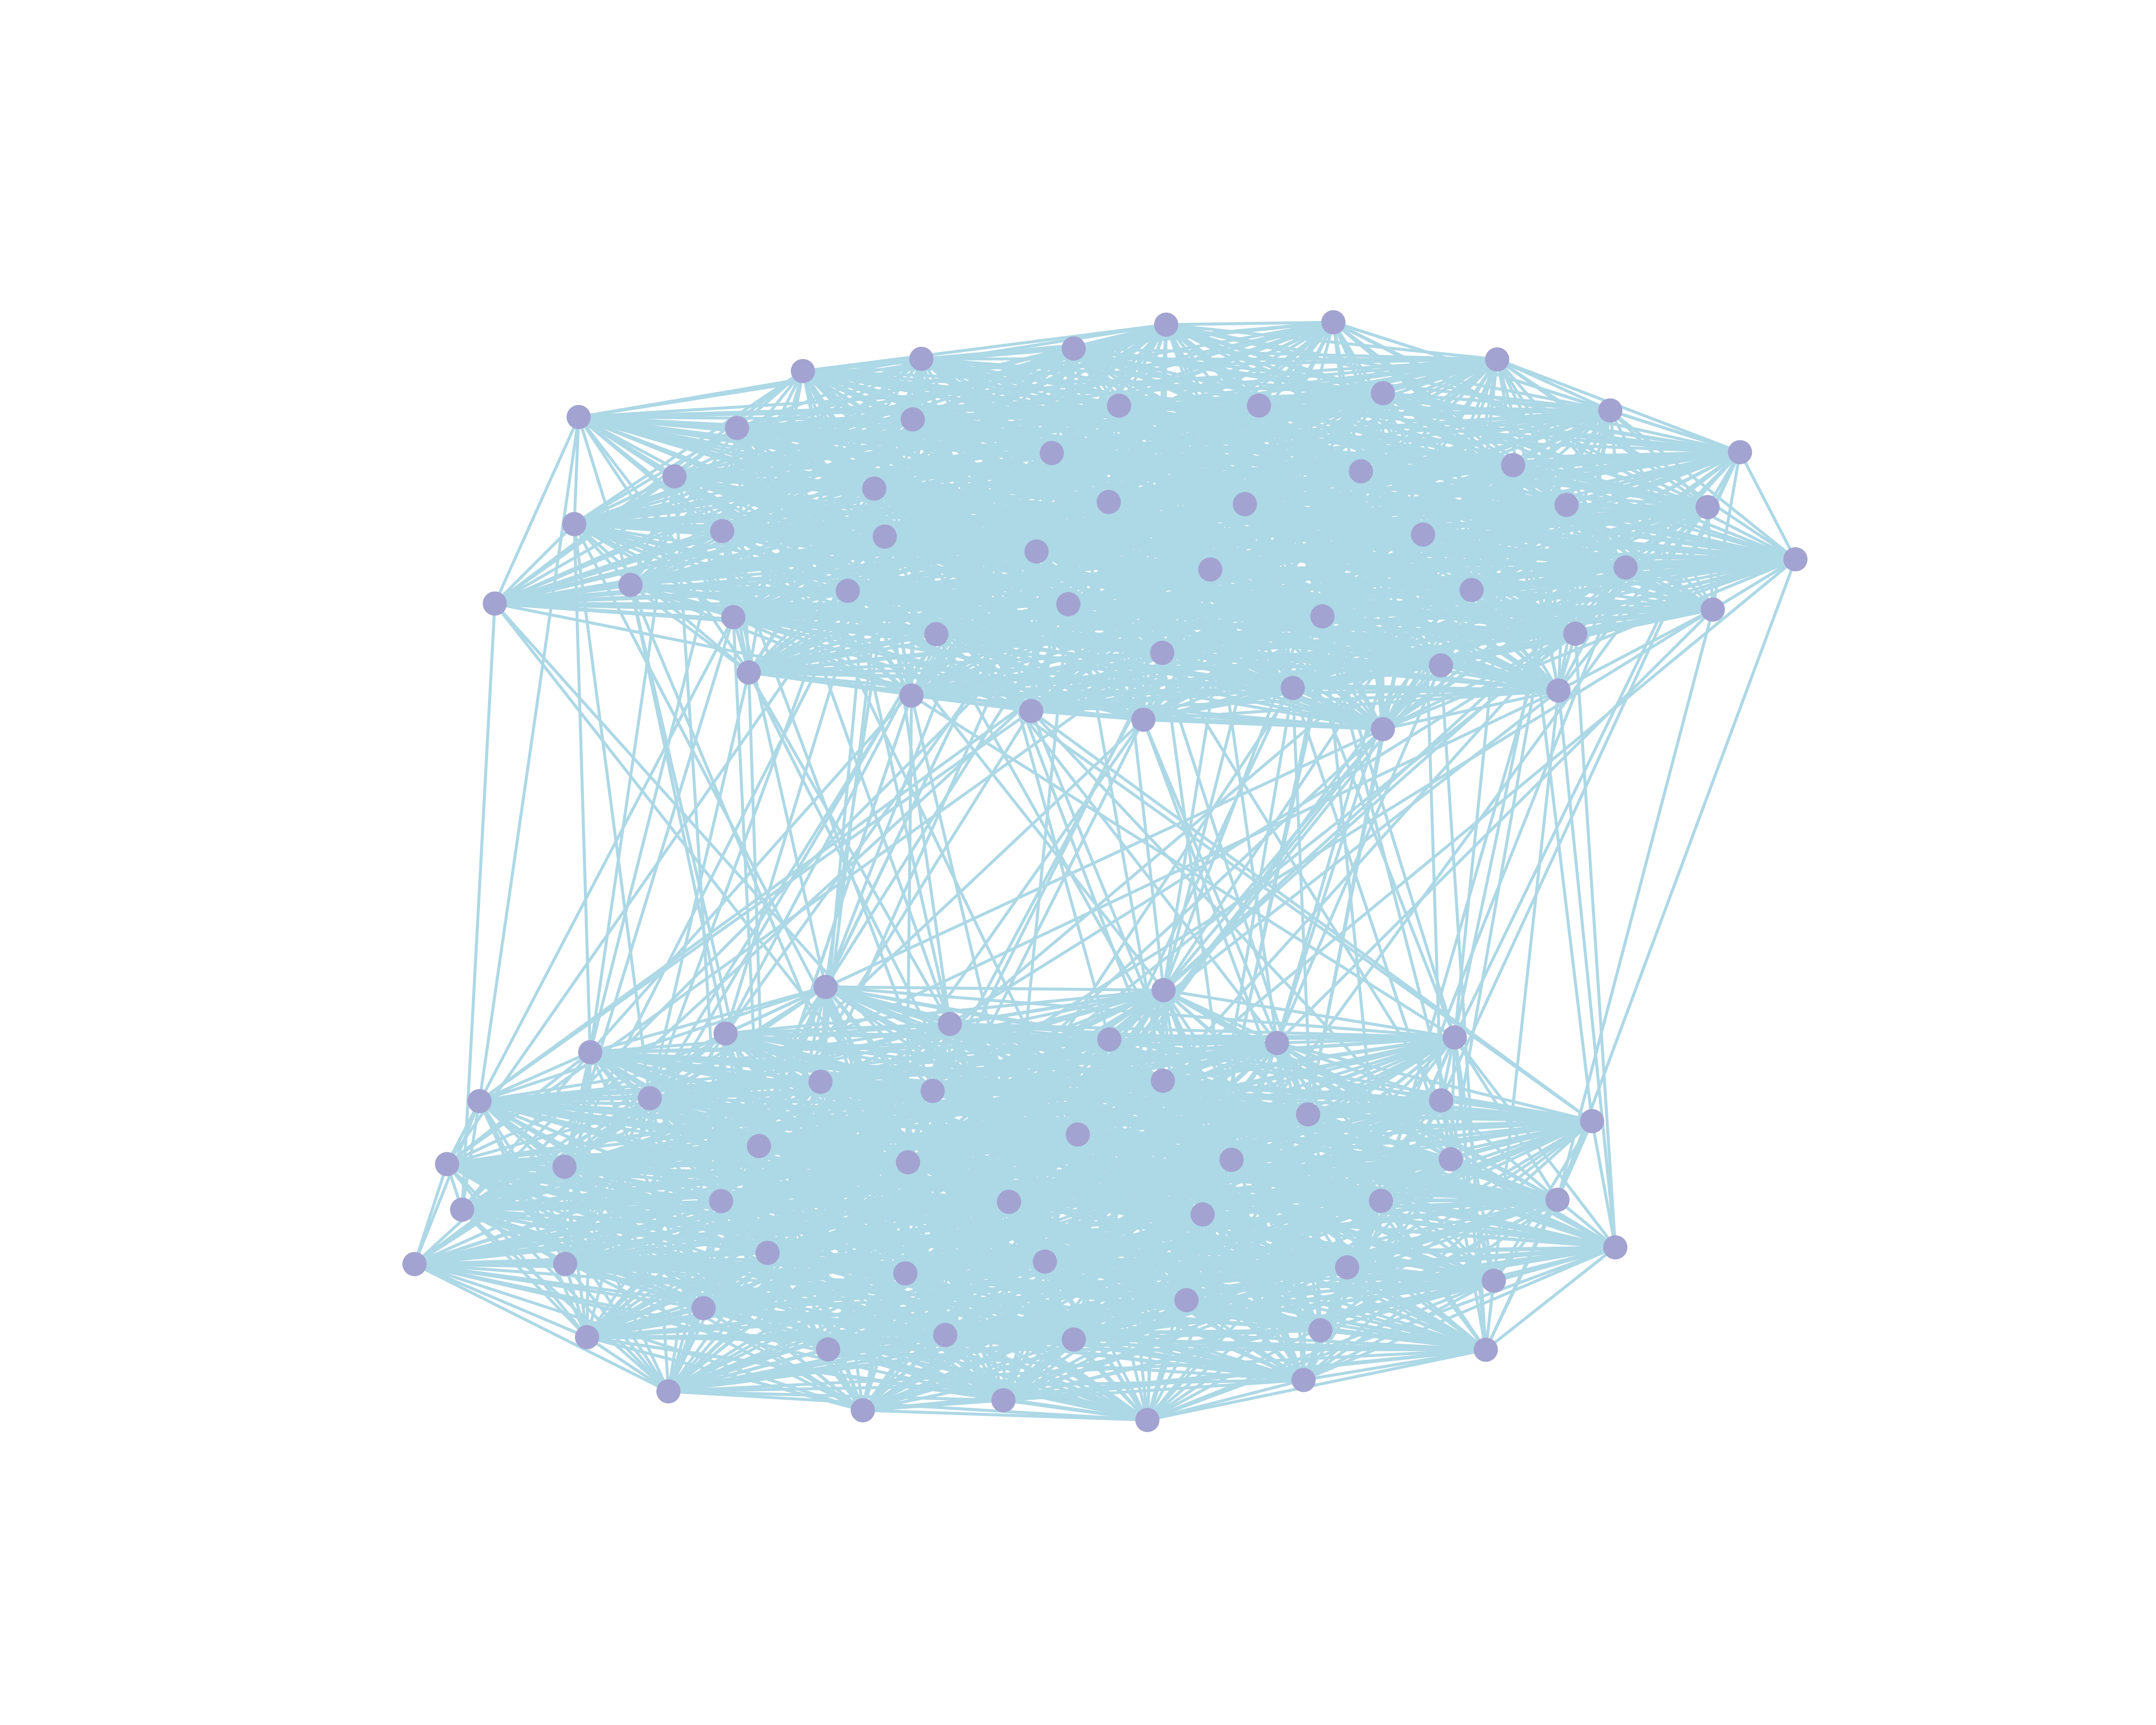
\includegraphics[width=\textwidth]{Graphics/ToyModelResults/SBM_results/BeforeRicciFlow.png}
        \caption{Initial SBM graph}
        \label{fig:sbm_initial}
    \end{subfigure}
    \hfill
    \begin{subfigure}[b]{0.45\textwidth}
        \centering
        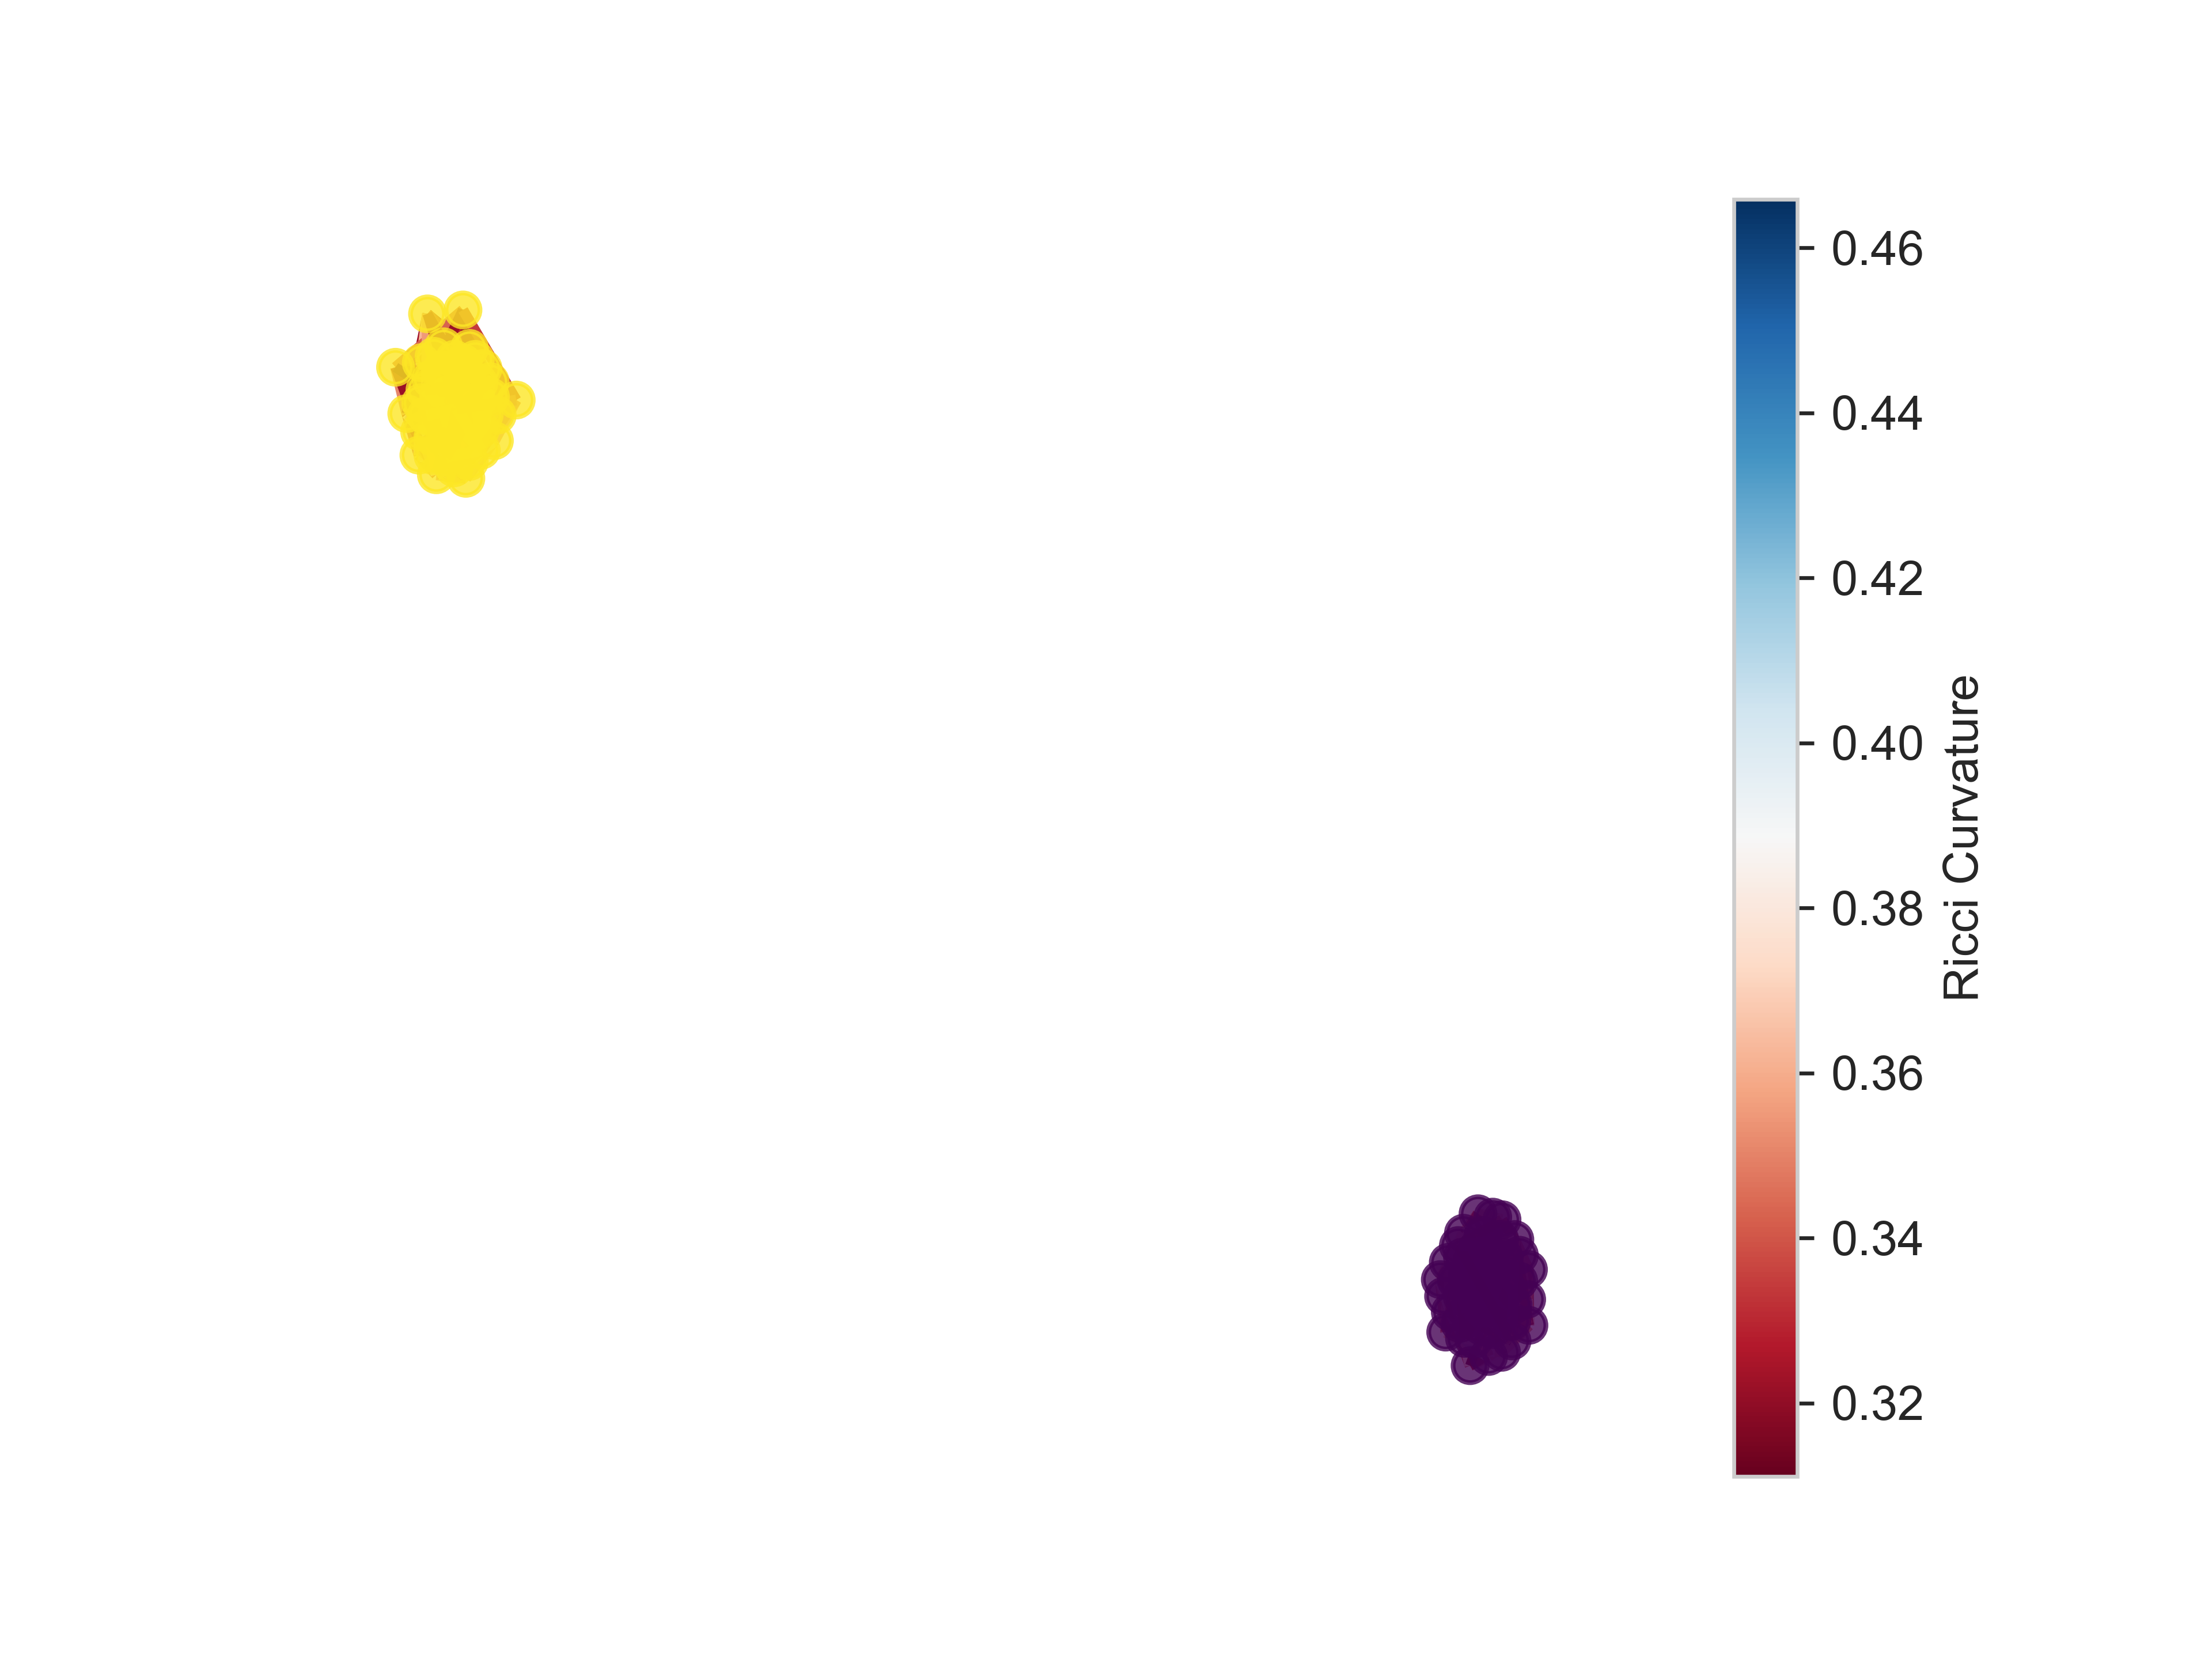
\includegraphics[width=\textwidth]{Graphics/ToyModelResults/SBM_results/Communities.png}
        \caption{Detected communities.}
        \label{fig:sbm_result}
    \end{subfigure}
    \caption{Comparison of the initial SBM graph and the community detection result.}
    \label{fig2}
\end{figure}

\begin{figure}[ht]
    \centering
    \begin{subfigure}[b]{0.45\textwidth}
        \centering
        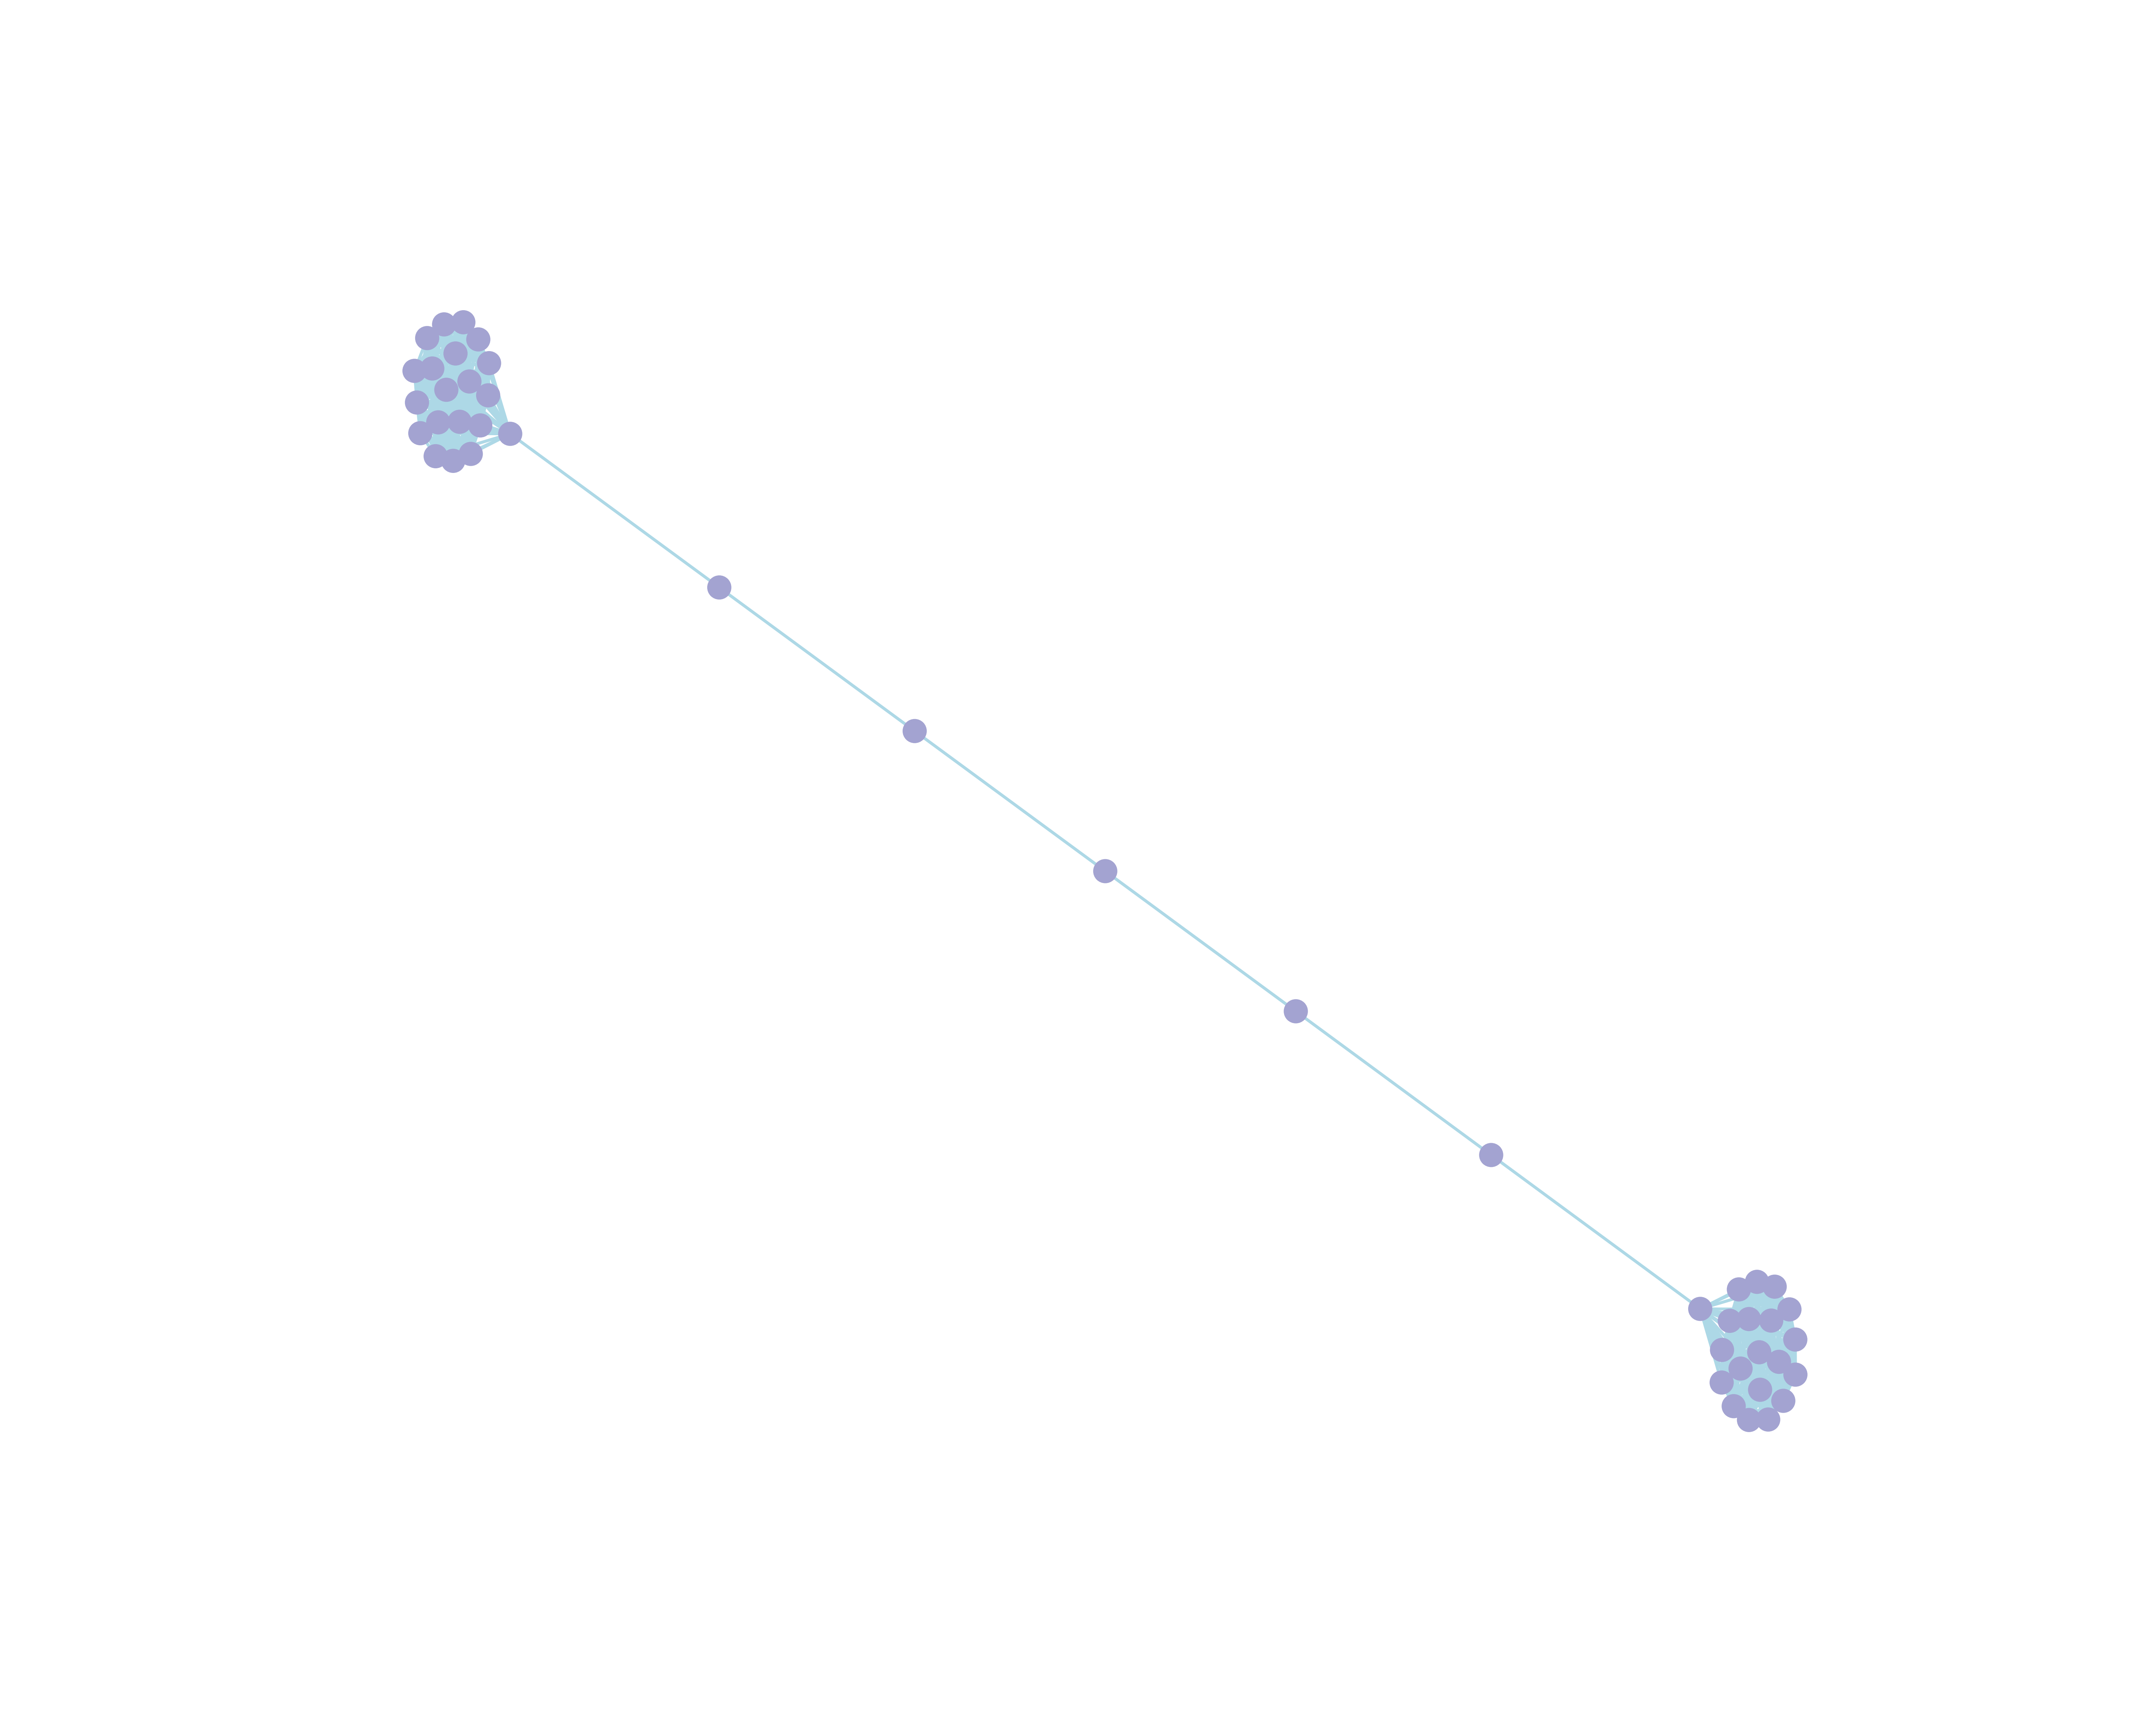
\includegraphics[width=\textwidth]{Graphics/ToyModelResults/Barbell_resluts/BeforeRicciFlow.png}
        \caption{Initial Barbell graph}
        \label{fig:barbell_initial}
    \end{subfigure}
    \hfill
    \begin{subfigure}[b]{0.45\textwidth}
        \centering
        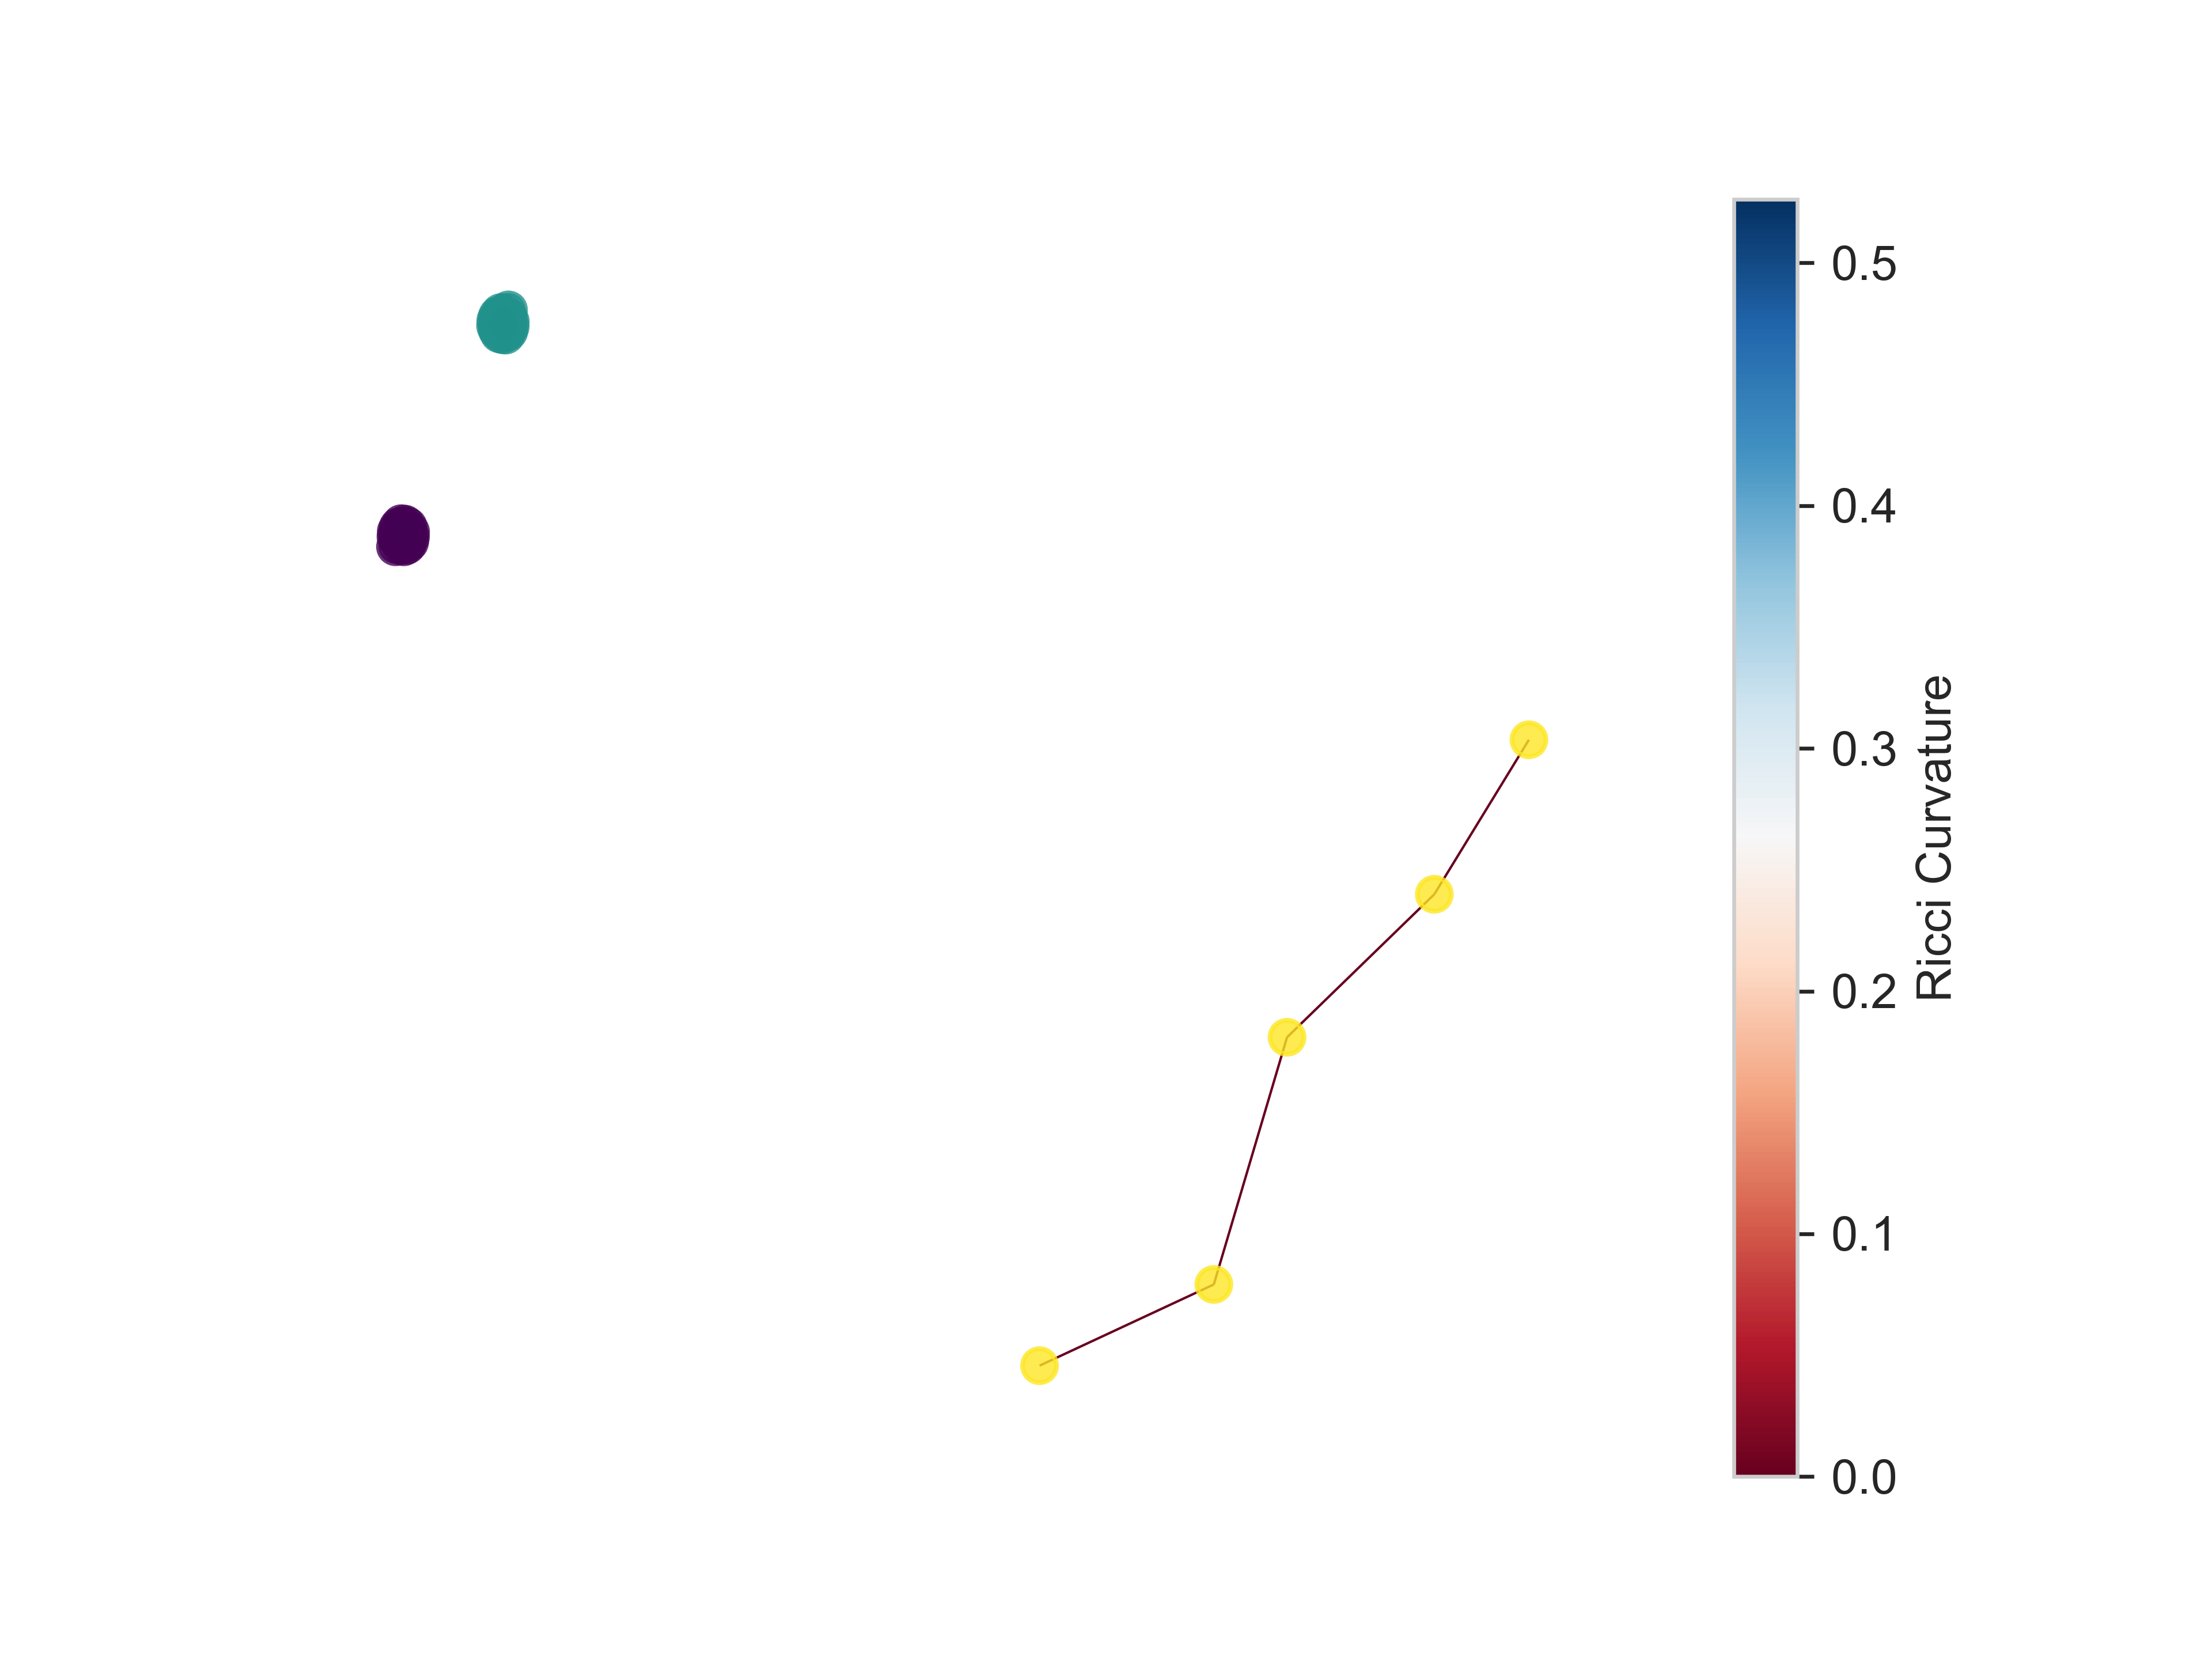
\includegraphics[width=\textwidth]{Graphics/ToyModelResults/Barbell_resluts/Communities.png}
        \caption{Detected communities}
        \label{fig:barbell_result}
    \end{subfigure}
    \caption{Comparison of the initial Barbell graph and the community detection result.}
    \label{fig3}
\end{figure}

\begin{figure}[ht!]
    \centering
    \begin{subfigure}[b]{0.45\textwidth}
        \centering
        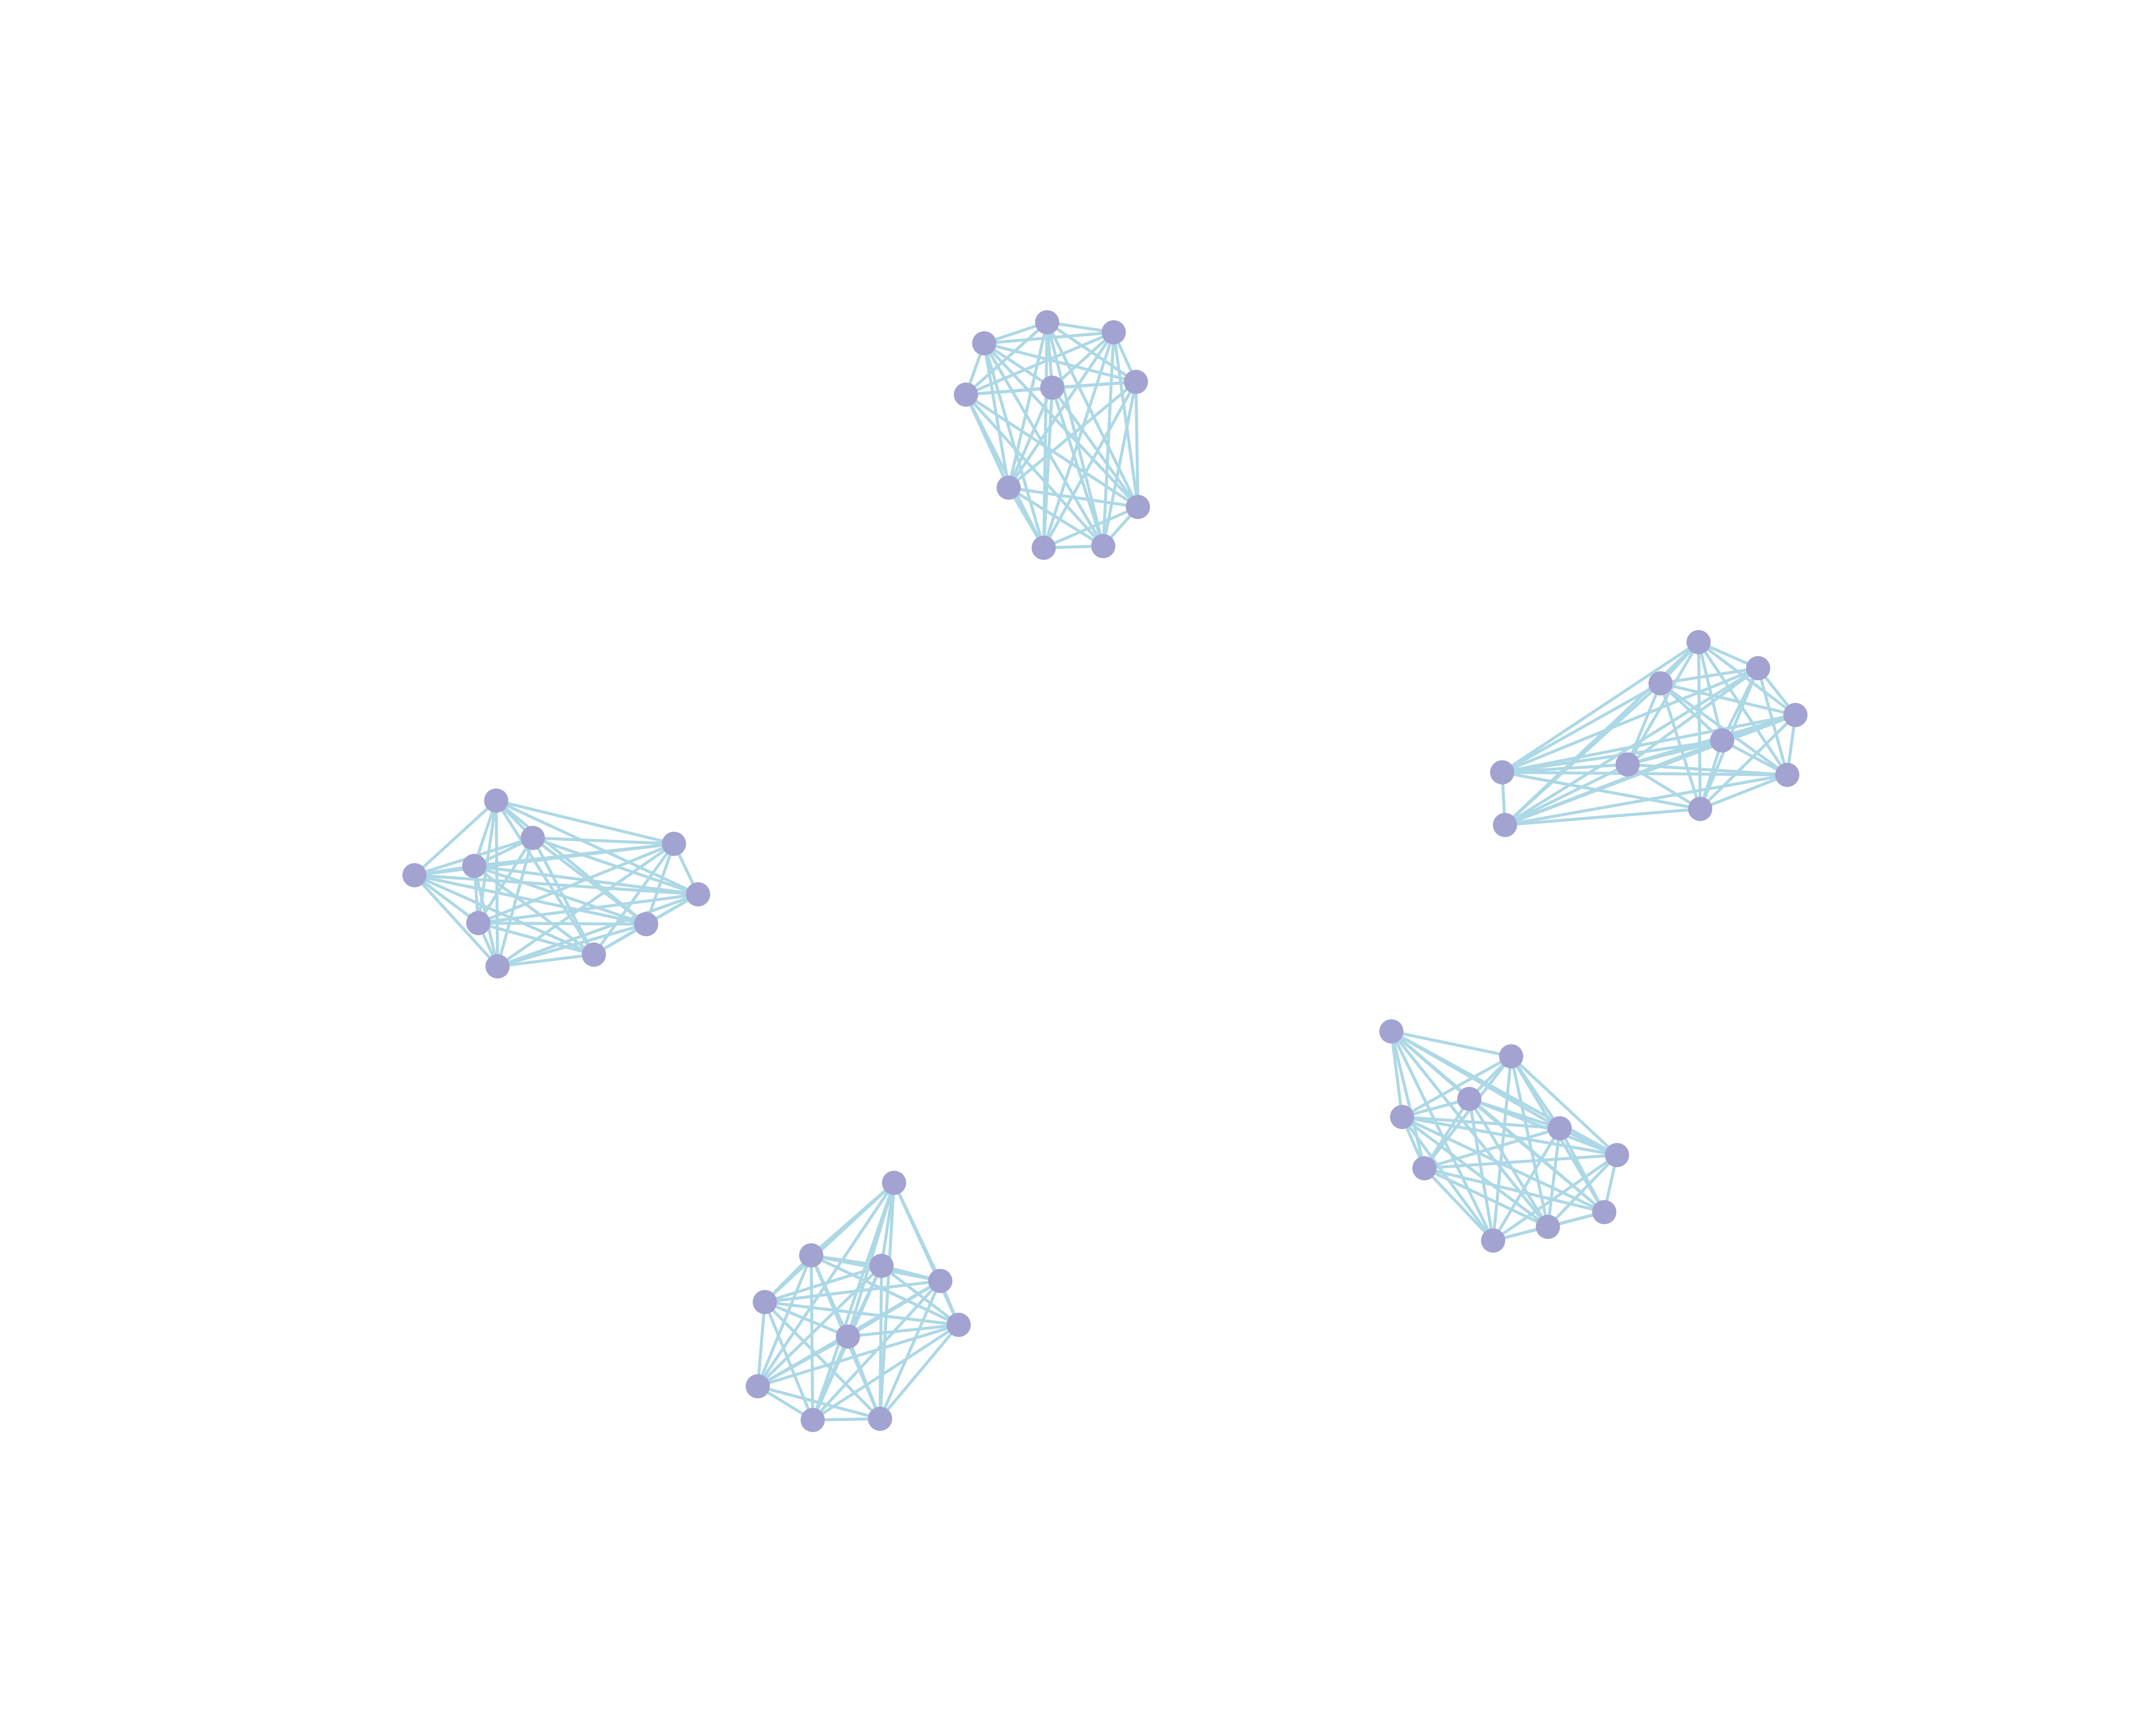
\includegraphics[width=\textwidth]{Graphics/ToyModelResults/Caveman_resluts/BeforeRicciFlow.png}
        \caption{Initial Caveman graph}
        \label{fig:caveman_initial}
    \end{subfigure}
    \hfill
    \begin{subfigure}[b]{0.45\textwidth}
        \centering
        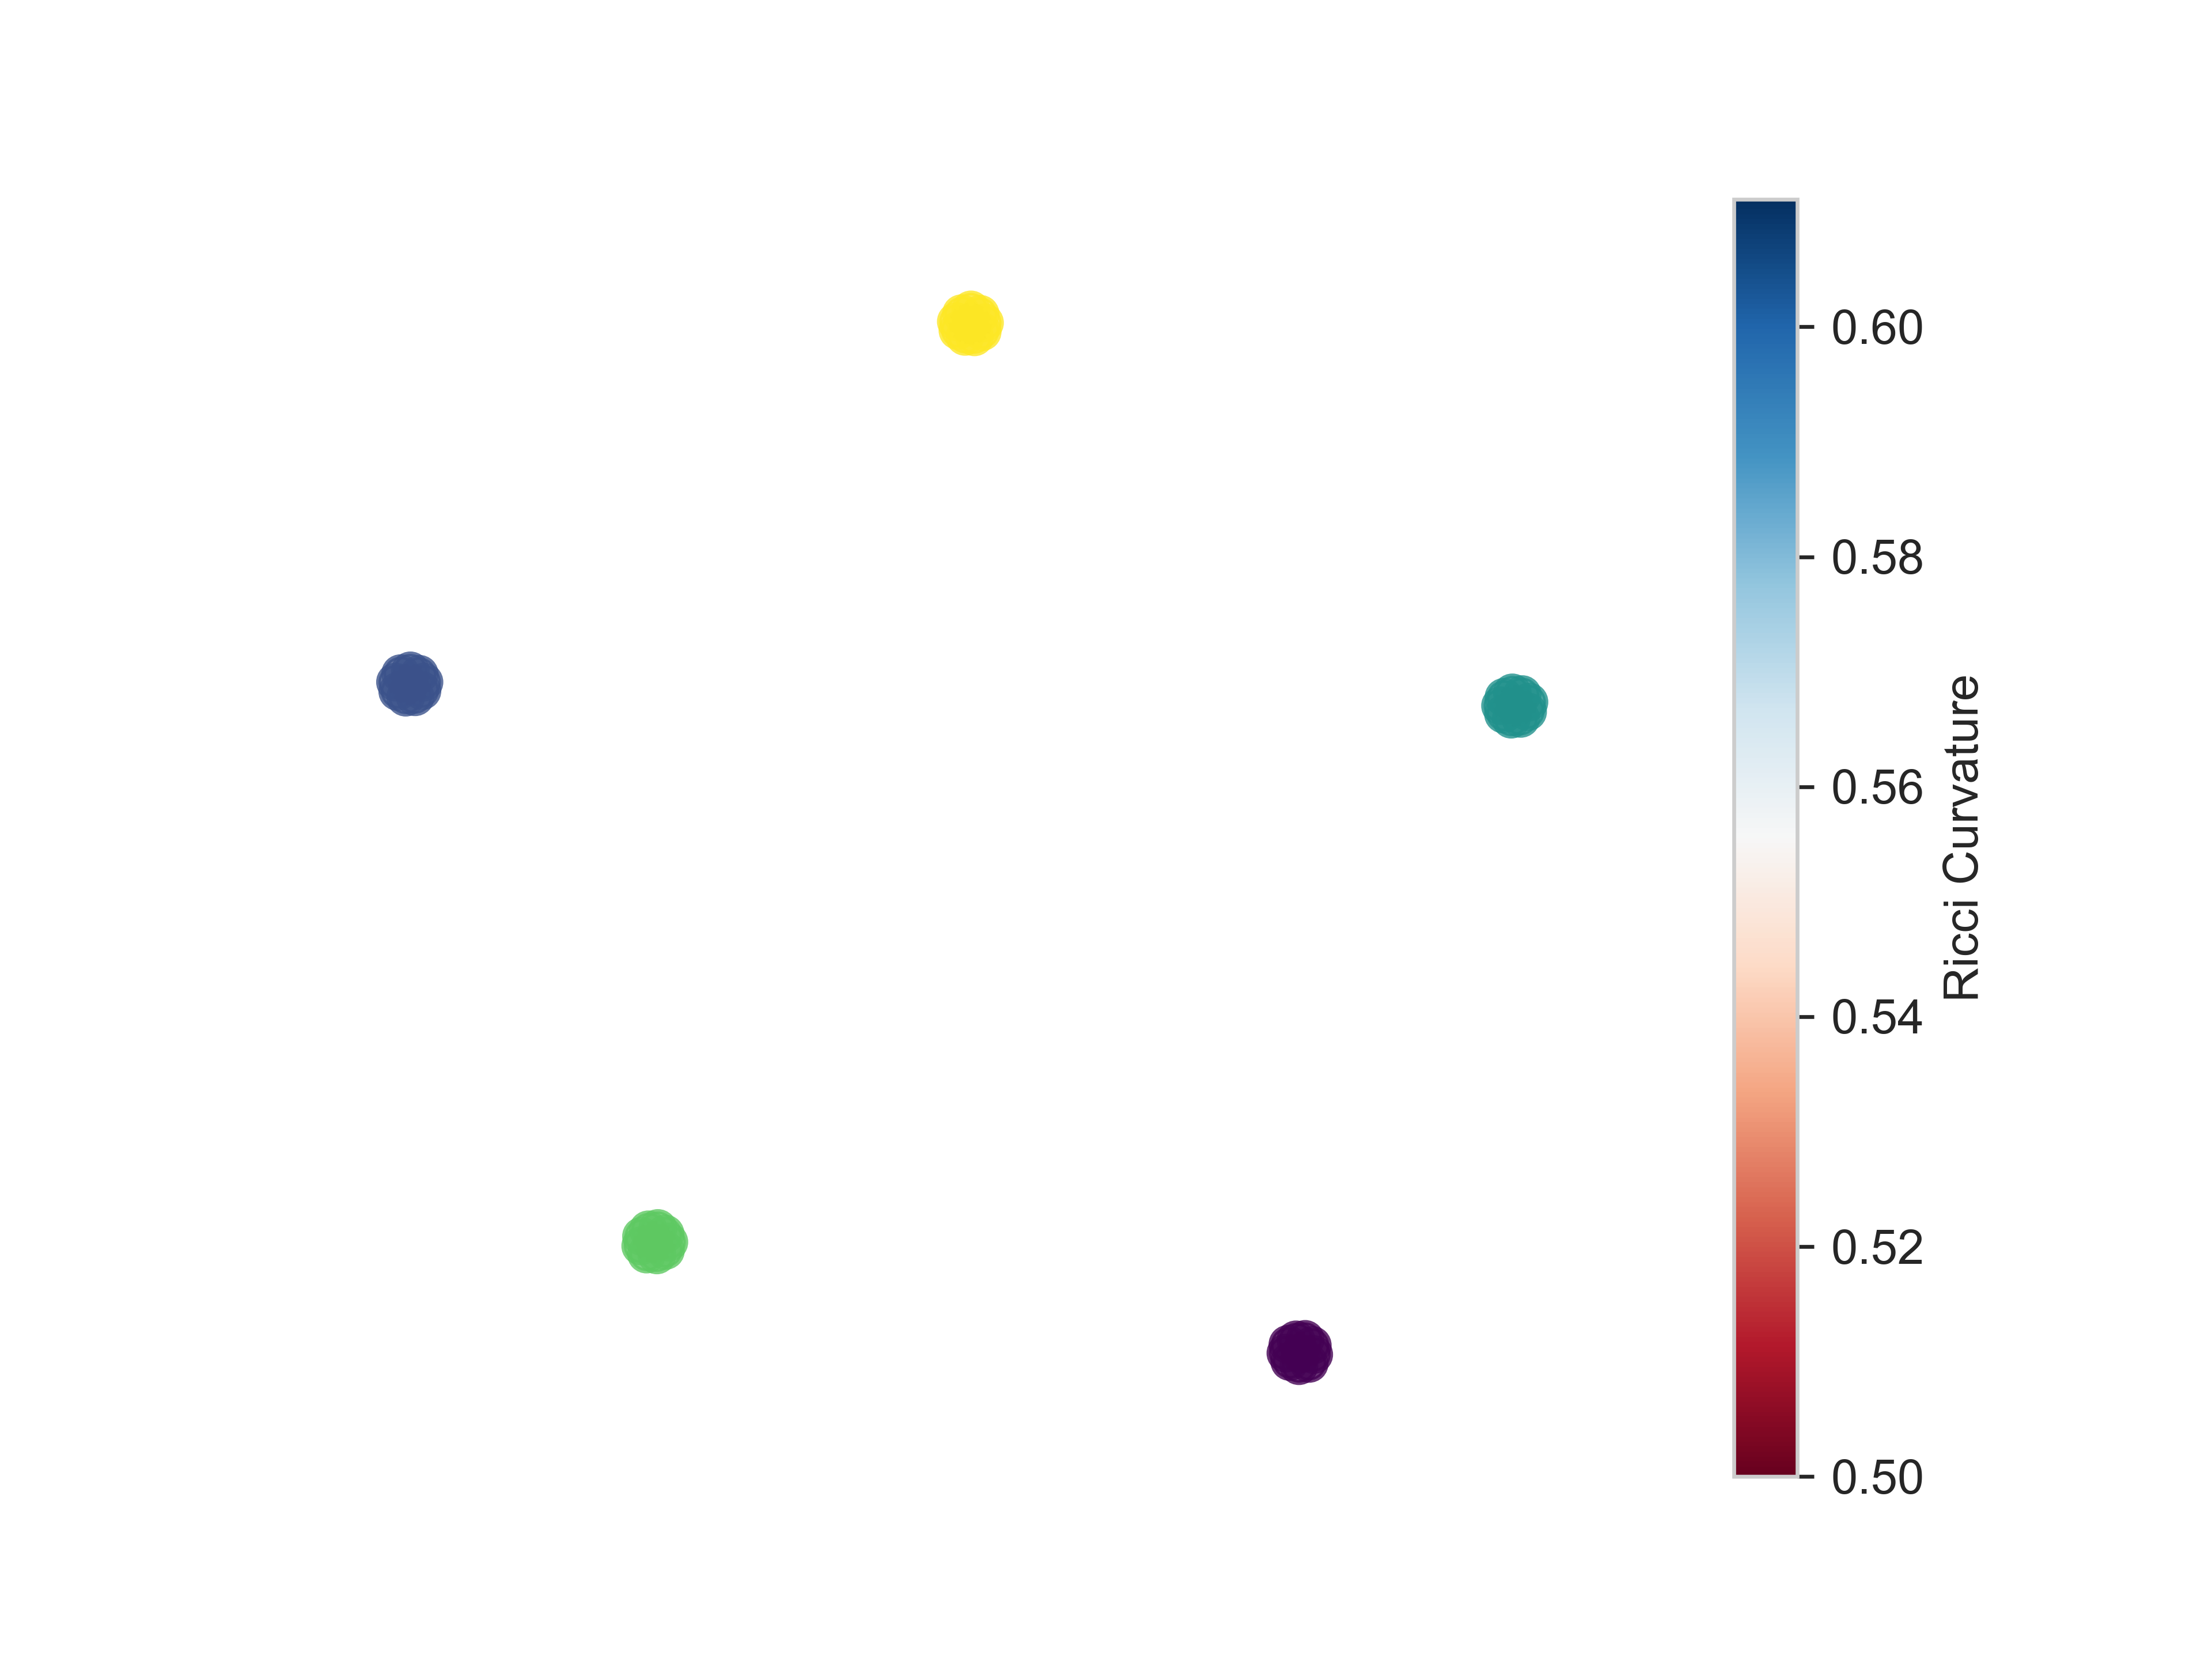
\includegraphics[width=\textwidth]{Graphics/ToyModelResults/Caveman_resluts/Communities.png}
        \caption{Detected communities}
        \label{fig:caveman_result}
    \end{subfigure}
    \caption{Comparison of the initial Caveman graph and the community detection result.}
    \label{fig4}
\end{figure}

\chapter{Implementation for Planar Graphs}
\section{Title}
\lipsum
\section{Results}
\lipsum

% ********************************** Appendices ********************************
\begin{appendices} % Using appendices environment for more functunality
\chapter{Metric of a 2-sphere}

%\section*{\hyperlink{Sphere}{Metric of a 2-sphere}} \label{appendix}
\begin{comment}
Start with the parameterisation of a 2-sphere with a radius $R$ and define the metric tensor $\eta$
\begin{equation*}
\centering
    \begin{cases}
      x = R \sin{(\theta)} \cos{(\phi)} \\
      y=  R \sin{(\theta)} \sin{(\phi)}\\
      z=  R \cos{(\theta)}
    \end{cases}
    \quad \text{and} \quad \eta_{ij} \equiv \begin{pmatrix}
\frac{\partial \Vec{x}}{\partial \theta} \frac{\partial \Vec{x}}{\partial \theta} & \frac{\partial \Vec{x}}{\partial \theta} \frac{\partial \Vec{x}}{\partial \phi} \\
\frac{\partial \Vec{x}}{\partial \phi}\frac{\partial \Vec{x}}{\partial \theta} & \frac{\partial \Vec{x}}{\partial \phi}\frac{\partial \Vec{x}}{\partial \phi} \\
\end{pmatrix}
\end{equation*}
\begin{equation*}
    \Rightarrow  \quad \eta_{ij}=\begin{pmatrix}
R^2 & 0 \\
0 & R^2 \sin^2(\theta) \\
\end{pmatrix}
\end{equation*}
where $\Vec{x}=\left( x , y , z \right)$. Now we can write the metric as
\begin{equation*}
    dl^2= \eta_{ij}\left( du^i , du^j \right) = R^2 \left( d\theta , d\phi \right) \begin{pmatrix}
1 & 0 \\
0 & \sin^2(\theta) \\
\end{pmatrix} \begin{pmatrix}
d\theta \\
d\phi \\
\end{pmatrix} = R^2 \left( d\theta^2 + \sin^2(\theta)d\phi^2 \right)
\end{equation*} 
where $\Vec{u}=(\theta,\phi)$.
\hspace*{\fill} $\Box$

\section*{\hyperlink{Ricci}{Components of the Ricci tensor for a generic spherically symmetric four dimensional metric}}
The explicit derivation will be shown only for the first component $R^0_0$, as the procedure is analogous for the others.

Starting from the expression of the Ricci tensor in terms of Christoffel symbols:
\begin{equation*}
    R^k {}_{\alpha k \beta} = \partial_\beta  \Gamma^k {}_{\alpha k} -\partial_k \Gamma^k {}_{\alpha \beta}+  \Gamma^\sigma {}_{\beta k} \Gamma^k {}_{\sigma \alpha}  -\Gamma^k {}_{k \sigma} \Gamma^\sigma {}_{\alpha \beta} 
\end{equation*}

we get 
\begin{align*}
    &R_{0 0} \equiv R^k {}_{0 k 0} =  \partial_0  \Gamma^k {}_{0 k}-\partial_k \Gamma^k {}_{0 0}  + \Gamma^\sigma {}_{0 k} \Gamma^k {}_{\sigma 0} - \Gamma^k {}_{k \sigma} \Gamma^\sigma {}_{0 0}   
\end{align*}

For the metric (\ref{eq2.1}), the terms that define $R_{00}$ are then expressed as
\begin{align*}
  \bullet \text{ } \Gamma^k {}_{0k} =& \partial_0 (\gamma + \alpha + 2\beta + \ln{\sin{\theta}}) = \Dot{\gamma} + \Dot{\alpha} +2\Dot{\beta} 
    \\ \rightarrow \quad \partial_0 \Gamma^k {}_{0k} =& \partial_0  (\Dot{\gamma} + \Dot{\alpha} +2\Dot{\beta})  = \Ddot{\gamma} + \Ddot{\alpha} +2\Ddot{\beta} \text{ ;}
    \\[15pt]  \bullet  \text{ } \Gamma^k {}_{0 0} =& \frac{1}{2} g^{k \nu} \left( g_{\nu 0 ,0} +  g_{\nu 0 ,0} -  g_{0 0,\nu} \right)= \frac{1}{2} g^{k\nu} \left(2g_{\nu 0,0}-g_{00,\nu}\right) 
  \\ =& \frac{1}{2}\left[ g^{k0}g_{0 0,0} + g^{k1}(2g_{0 1,0} - g_{0 0,1})\right] = \frac{1}{2}\left[ g^{k0}g_{0 0,0} - g^{k1} g_{0 0,1}\right] 
   \\ \rightarrow \quad \partial_k \Gamma^k {}_{00} =& \partial_0 \frac{1}{2}\left( e^{-2\gamma}2\dot{\gamma}e^{2\gamma}\right) - \partial_1 \frac{1}{2}\left(-e^{-2\alpha} 2\gamma^\prime e^{2\gamma}\right)
   \\ =& \Ddot{\gamma} + e^{2\gamma-2\alpha}\left(\gamma^{\prime \prime}+2{\gamma^\prime}^2 -2 \gamma^\prime \alpha^\prime \right) \text{;}
    \\[15pt]  \bullet \text{ } \Gamma^\sigma {}_{0 k} =& \frac{1}{2} g^{\sigma \nu} \left( g_{\nu 0, k} + g_{\nu k, 0} - g_{0 k, \nu}\right) 
    \\=& \frac{1}{2} \left[g^{\sigma 0} \left(  g_{0 0, k} + g_{0 k, 0} - g_{0 k, 0}\right) + g^{\sigma 1} \left( g_{1 0, k} + g_{1 k, 0} - g_{0 k, 1}\right) \right]
    \\ \Gamma^k {}_{\sigma 0} =& \frac{1}{2} g^{k \nu} \left( g_{\nu \sigma, 0} + g_{\nu 0,\sigma} - g_{\sigma 0, \nu}\right) 
    \\=& \frac{1}{2} \left[g^{k 0} \left( g_{0 \sigma, 0} + g_{0 0, \sigma} + - g_{\sigma 0, 0}\right) + g^{k 1}\left( g_{0 1, \sigma} + g_{\sigma 1, 0} - g_{\sigma 0, 1}\right) \right]
    \\ \rightarrow \quad \Gamma^\sigma {}_{0 k} \Gamma^k {}_{\sigma 0}  =& \Gamma^0 {}_{0 0} \Gamma^0 {}_{0 0} + \Gamma^0 {}_{0 1} \Gamma^1 {}_{0 0} + \cancel{\Gamma^0 {}_{0 2} \Gamma^2 {}_{0 0}} + \cancel{\Gamma^0 {}_{0 3} \Gamma^3 {}_{0 0}} + \Gamma^1 {}_{0 0} \Gamma^0 {}_{1 0} + \Gamma^1 {}_{0 1} \Gamma^1 {}_{1 0} 
    \\ +&\cancel{\Gamma^1 {}_{0 2} \Gamma^2 {}_{1 0}} + \cancel{\Gamma^1 {}_{0 3} \Gamma^3 {}_{1 0}} + \cancel{\Gamma^2 {}_{0 0} \Gamma^0 {}_{2 0}} + \cancel{\Gamma^2 {}_{0 1} \Gamma^1 {}_{2 0}} + \Gamma^2 {}_{0 2} \Gamma^2 {}_{2 0} + \cancel{\Gamma^2 {}_{0 3} \Gamma^3 {}_{2 0}} 
    \\ +&\cancel{\Gamma^3 {}_{0 0} \Gamma^0 {}_{3 0}} + \cancel{\Gamma^3 {}_{0 1} \Gamma^1 {}_{3 0}} + \cancel{\Gamma^3 {}_{0 2} \Gamma^2 {}_{3 0}}  + \Gamma^3 {}_{0 3} \Gamma^3 {}_{3 0} 
    \\ =& \Dot{\gamma}^2 + {\gamma^\prime}^2 e^{2\gamma-2\alpha} + {\gamma^\prime}^2 e^{2\gamma-2\alpha}+ \Dot{\alpha}^2 + \Dot{\beta}^2 + \Dot{\beta}^2
    \\ =& \dot{\gamma}^2 + \dot{\alpha}^2 + 2 \dot{\beta}^2 + 2{\gamma^\prime}^2 e^{2\gamma-2\alpha} \text{ ;}
    \\[15pt]  \bullet \text{ } \Gamma^\sigma 
    {}_{0 0} =&  \frac{1}{2} g^{\sigma \nu}(2g_{\nu 0,0} - g_{00,\nu})  
    = \frac{1}{2} \left[ g^{\sigma 0}g_{00,0} -g^{\sigma 1}g_{00,1}\right]
    \\ \Gamma^k {}_{k \sigma} =& \partial_\sigma (\gamma + \alpha +2\beta + \ln{\sin{\theta}})
    \\ \rightarrow \quad  \Gamma^k {}_{k \sigma} \Gamma^\sigma {}_{0 0} =& \frac{1}{2} e^{-2\gamma}\left(2 \Dot{\gamma}e^{2\gamma}\right)  \left(\Dot{\gamma} + \Dot{\alpha} +2\Dot{\beta} \right) - \frac{1}{2} e^{-2\alpha}\left(- 2 \gamma^\prime e^{2\gamma}\right)  \left(\gamma^\prime +\alpha^\prime +2\beta^\prime \right)
    \\ =&\dot{\gamma}^2 + \dot{\gamma}\Dot{\alpha} + 2\dot{\gamma}\Dot{\beta} + e^{2\gamma-2\alpha}\left({\gamma^\prime}^2+ \gamma^\prime \alpha^\prime + 2\gamma^\prime \beta^\prime \right)
\end{align*}
where dots and primes stand for $\frac{\partial}{\partial t}$ and  $\frac{\partial}{\partial r}$, respectively. 
In the computation we made use of two important relationships that hold in the case of a symmetric connection: 
\begin{equation*}
    \Gamma^\mu {}_{\alpha \beta} = \frac{1}{2} g^{\mu \nu} \left( g_{\nu \alpha,\beta} + g_{\nu \beta,\alpha} -  g_{\alpha \beta,\nu} \right) \quad \text{and} \quad \Gamma^\alpha {}_{\mu \alpha} = \Gamma^\alpha {}_{\alpha \mu} = \partial_\mu \left( \ln{\sqrt{-g}}\right)
\end{equation*}
Where the term $\ln{\sqrt{-g}} \equiv \ln{\sqrt{-\det g_{\mu \nu}}}$ evaluates as
\begin{align*}
    g  &= -e^{2\gamma + 2\alpha +4\beta}\sin^2{\theta}
    \\ \sqrt{-g} &= e^{\gamma + \alpha +2\beta}\sin{\theta}
    \\ \ln{\sqrt{-g}} &=\gamma + \alpha +2\beta + \ln{\sin{\theta}}
\end{align*}

We are now able to write
\begin{align*}
    R_{00} =& \text{ } \Ddot{\gamma} + \Ddot{\alpha} + 2\Ddot{\beta} - \Ddot{\gamma} - e^{2\gamma-2\alpha}\left(\gamma^{\prime \prime}+2{\gamma^\prime}^2 -2 \gamma^\prime \alpha^\prime \right) + \dot{\gamma}^2 + \dot{\alpha}^2 + 2 \dot{\beta}^2 + {\gamma^\prime}^2 e^{2\gamma-2\alpha}
    \\ -& \dot{\gamma}^2 - \dot{\gamma}\Dot{\alpha} - 2\dot{\gamma}\Dot{\beta} 
     - e^{2\gamma-2\alpha}\left({\gamma^\prime}^2+ \gamma^\prime \alpha^\prime + 2\gamma^\prime \beta^\prime \right)
    \\ =& \text{ } \Ddot{\alpha} + 2\Ddot{\beta} + 2 \dot{\beta}^2  -
    \Dot{\gamma} \left( \Dot{\alpha} + 2\Dot{\beta} \right) + \dot{\alpha}^2 - e^{2\gamma-2\alpha}\left( \gamma^{\prime \prime} - \gamma^\prime \alpha^\prime + {\gamma^\prime}^2 + 2\gamma^\prime \beta^\prime\right)
\end{align*}
To obtain $R^0_0$ we use the relationship $R^0_0=g^{0 0}R_{0 0}$, where $g^{0 0} = e^{-2\gamma}$. 
\begin{equation*}
    R^0_0=e^{-2\gamma}\left[ 2 \Ddot{\beta} + \Ddot{\alpha} + 2 \dot{\beta}^2 + \dot{\alpha}^2 - \dot{\gamma} \left( 2 \dot{\beta} + \dot{\alpha} \right) \right] - e^{-2 \alpha}\left[ \gamma^{\prime \prime} + \gamma^{\prime} \left( 2 \beta^\prime + \gamma^\prime - \alpha^\prime \right) \right]
\end{equation*}
\hspace*{\fill} $\Box$
\end{comment}
\end{appendices}

% ********************************** Back Matter *******************************
% Backmatter should be commented out, if you are using appendices after References
\backmatter

% ********************************** Bibliography ******************************
\begin{spacing}{0.9}

\cleardoublepage
\nocite{*}
\printbibliography[heading=bibintoc, title={References}]

\end{spacing}

% ******************************************************************************
% ******************************** END DOCUMENT ********************************
% ******************************************************************************

\end{document}